\documentclass[11pt,letterpaper]{article}
\usepackage[T1]{fontenc}
\usepackage[utf8]{inputenc}
\usepackage{mathpazo}
\usepackage[margin=1.05in]{geometry}
\usepackage{microtype}
\usepackage{amsmath,amssymb,amsthm,mathtools,mathrsfs}
\usepackage{booktabs,array,graphicx}
\usepackage{tikz}
\usetikzlibrary{arrows.meta,decorations.pathreplacing}
\usepackage[numbers,sort&compress]{natbib}
\usepackage{xcolor}
\definecolor{linkblue}{RGB}{25,65,112}
\usepackage[colorlinks=true,linkcolor=linkblue,citecolor=linkblue,urlcolor=linkblue]{hyperref}
\urlstyle{same}
\hypersetup{pdftitle={Quantitative lower bounds for trace reconstruction},pdfauthor={OpenAI},pdfsubject={Quantitative lower bounds for full binary deletion traces},pdflang={en-US}}
\pdftrailerid{}
\pdfsuppressptexinfo=15
\numberwithin{equation}{section}
\newtheorem{theorem}{Theorem}[section]
\newtheorem{proposition}[theorem]{Proposition}
\newtheorem{lemma}[theorem]{Lemma}
\newtheorem{corollary}[theorem]{Corollary}
\theoremstyle{definition}
\newtheorem{definition}[theorem]{Definition}
\theoremstyle{remark}
\newtheorem{remark}[theorem]{Remark}
\DeclareMathOperator{\TV}{TV}
\DeclareMathOperator{\ov}{ov}
\DeclareMathOperator{\supp}{supp}
\DeclareMathOperator{\popcount}{popcount}
\DeclareMathOperator{\Bin}{Bin}
\newcommand{\Dcal}{\mathcal D}
\newcommand{\E}{\mathbb E}
\newcommand{\Prob}{\mathbb P}
\newcommand{\Id}{I}
\newcommand{\norm}[1]{\lVert #1\rVert}
\newcommand{\abs}[1]{\lvert #1\rvert}
\newcommand{\R}{\mathbb R}
\newcommand{\N}{\mathbb N}
\setlength{\emergencystretch}{2em}
\allowdisplaybreaks[2]

\newcommand{\QL}{\Lambda}
\newcommand{\Ber}{\mathrm{Ber}}
\newcommand{\Tr}{\mathrm{Tr}}

\title{Quantitative lower bounds for trace reconstruction}
\author{OpenAI}
\date{September 24, 2026}
\begin{document}
\maketitle
\begin{abstract}
Exact worst-case reconstruction of a binary word from independent deletion traces requires $n^{\Omega(\log\log n)}$ samples for every fixed deletion probability $q\in(0,1)$, even with unrestricted computation and any fixed positive success probability. This gives a negative answer to the polynomial-sample question for binary trace reconstruction. More generally, when $q^3\log n\to\infty$, we prove a lower bound of $n^{c\log(q^3\log n)}$ samples for every fixed $0<c<1/(4\log2)$. Here $q$ is the known deletion probability, and all logarithms are natural.
\end{abstract}
\section{Introduction}\label{sec:introduction}

For a binary word $x$ and a known deletion probability $q\in(0,1)$, let $\Dcal_q(x)$ denote the law obtained by deleting each bit independently with probability $q$ and concatenating the surviving bits in their original order.  The retention probability is $p=1-q$.  A sample from this law is a \emph{complete trace}: its length and all surviving bits are observed, without the positions they occupied in $x$.

For $s\in(0,1]$, let $T_{q,s}(n)$ be the least nonnegative integer $m$ for which an estimator, given $n,q$ and $m$ independent complete traces, recovers every $x\in\{0,1\}^n$ with probability at least $s$.  The estimator may be randomized and its computation is unrestricted.  If no finite $m$ suffices, set $T_{q,s}(n)=+\infty$.  Write $T_q(n)=T_{q,2/3}(n)$.  Our lower bounds concern this fixed sample budget.

\begin{theorem}[Quantitative sample lower bound]\label{thm:main}
Fix $s\in(0,1]$ and $0<c<1/(4\log2)$.  Along every sequence of instances $(n,q)$ with $n\to\infty$, $q\in(0,1)$, and $q^3\log n\to\infty$,
\begin{equation}\label{eq:main-bound}
 T_{q,s}(n)\ge n^{c\log(q^3\log n)}
\end{equation}
eventually.  All logarithms are natural.  In particular, for each fixed deletion probability $q\in(0,1)$ and fixed positive success probability $s$, the required sample number is $n^{\Omega(\log\log n)}$.
\end{theorem}

The varying-channel statement keeps the requested channel fixed throughout the construction for each instance; it is allowed to change only when the instance changes.  The result gives a negative answer to the polynomial-sample question for deterministic binary inputs at every fixed deletion probability.  A separate consequence concerns one-trace indistinguishability itself.  For laws on the countable set of finite binary words, write
\[
 \TV(P,Q)=\frac12\sum_w|P(w)-Q(w)|.
\]

\begin{theorem}[Superpolynomial one-trace indistinguishability]\label{thm:tv}
For every fixed deletion probability $q\in(0,1)$,
\begin{equation}\label{eq:min-tv}
 \lim_{n\to\infty}n^A
 \min_{\substack{x,y\in\{0,1\}^n\\x\ne y}}
 \TV\bigl(\Dcal_q(x),\Dcal_q(y)\bigr)=0
 \qquad\text{for every }A>0.
\end{equation}
At this same channel $T_{q,s}(n)/n^A\to\infty$ for every fixed $A>0$ and $s\in(0,1]$.
\end{theorem}

The channel is fixed independently of $A$.  The proof of \eqref{eq:min-tv} uses an explicit score and approximation bound.  Since the minimum is attained at every $n$, a single sequence of minimizing pairs realizes all the limits simultaneously.

\subsection{History and comparison with earlier results}

Reconstructing a sequence from repeated corrupted observations has a long history.  Levenshtein studied both combinatorial and memoryless channel formulations \citep{Levenshtein2001}.  Batu, Kannan, Khanna, and McGregor studied the independent-deletion trace problem in connection with multiple sequence alignment and outlined a linear sample obstruction at fixed deletion probability \citep[Section 4.2]{Batu2004}.  Later lower bounds for complete traces focused on the difficulty of locating a small discrepancy within a long background.  McGregor, Price, and Vorotnikova analyzed neighboring positions of a single one among zeros, using Hellinger distance and common mass \citep{MPV2014}.  Holden and Lyons used a defect in an alternating background to prove $\Omega(n^{5/4}/\sqrt{\log n})$ \citep{HoldenLyons2020,HoldenLyonsErratum2022}, and Chase obtained $\Omega(n^{3/2}/\log^7 n)$ by a direct Hellinger calculation for a related pair \citep{Chase2021Lower}.  The displayed Holden--Lyons and Chase rates fix the channel and a reconstruction success greater than $1/2$.  Our seed starts from the periodic defect family used by Chase and makes signed choices across many periods; it also supplies the overlap and score estimates needed for repeated amplification.

For fixed deletion probability, Holenstein, Mitzenmacher, Panigrahy, and Wieder obtained a worst-case upper bound of $\exp(\widetilde O(\sqrt n))$ \citep{HMPW2008}, where $\widetilde O$ suppresses polylogarithmic factors.  Independently, De, O'Donnell, and Servedio and Nazarov and Peres improved it to $\exp(O(n^{1/3}))$ \citep{DOS2017,NP2017}, and Chase obtained $\exp(O(n^{1/5}\log^5 n))$ \citep{Chase2021Upper}.  The 2026 preprint of Burudgunte, Valiant, and Wang gives
$\exp(p^{-7/3}(\log_2 n)^{C_0})$ samples for a universal constant $C_0$ and every positive retention probability $p=1-q$ \citep{BVW2026}.  At fixed $p$ this is a quasipolynomial sample upper bound; the cited preprint does not give a quasipolynomial-time reconstruction algorithm.  The logarithm of this sample bound is a fixed power of $\log n$, whereas the logarithm of our lower bound at a fixed channel has order $(\log n)(\log\log n)$, leaving a gap between the rates.  The companion paper \emph{Uniform quasipolynomial-time trace reconstruction} proves such a time bound for every fixed known rational retention probability \citep{OAI:Uniform-quasipolynomial-time-trace-reconstruction-October-5-2026}.

Polynomial reconstruction remains possible under other channel or input conditions.  For every fixed $\varepsilon>0$, Chen, De, Lee, Servedio, and Sinha give reconstruction in polynomial time when $q\le n^{-1/3-\varepsilon}$, using $O(n^{4/3})$ traces \citep{CDLSS2021LowDeletion}.  Those deletion probabilities lie outside the regime $q^3\log n\to\infty$ of Theorem~\ref{thm:main}.  Aamand, Liu, and Narayanan prove polynomial reconstruction when the internal zero gaps between successive ones have length at least a sufficiently large constant times $(\log n)^8$ and the deletion probability is at most a sufficiently small universal constant \citep{ALN2025}.

Some lower bounds restrict the available statistics.  De, O'Donnell, and Servedio measure the precision required of an oracle returning an $\ell^1$ approximation to the expected trace vector padded with zeros, while Nazarov and Peres study repeated observations of one fixed output coordinate \citep{DOS2017,NP2017}.  Chen, De, Lee, and Servedio study a tolerance oracle for functions of contiguous blocks of trace coordinates \citep{CDLS2024}.  Their lower bounds concern those specified statistics.  A different input model is studied by Rivkin, Valiant, and Valiant: the input is a fixed probability vector, with fresh Bernoulli bits drawn from it before each trace.  For deletion probability at least a constant times $n^{-1/2}$, their generalized trace laws can have total variation $\exp(-\Omega(\sqrt n))$ \citep{RivkinValiantValiant2025}.  Their arguments using translated segments and cancellation are related to the observation constructed in Section~\ref{sec:layout}.  Theorems~\ref{thm:main} and~\ref{thm:tv} concern the entire trace law of one deterministic binary word.

\subsection{Mechanism and proof structure}

Our construction hides differences in location at several scales.  The basic source of hidden randomness is exact common mass.  If trace laws for $k$ and $k+1$ copies of a word share mass $\omega$, place such a pair of runs on opposite sides of a central segment and choose their orientation by a fair bit.  Their joint trace laws share a product component of mass $\omega^2$.  On that component the orientation remains fair even after the side outputs are reported.  Many independent pairs therefore leave a binomial uncertainty in the position of the central segment.  Marginalizing the flags restores the product of the two side trace laws for each orientation.  Concatenating independent genuine traces of a partition of the fixed word then recovers its trace law exactly.  At later scales the preliminary observation uses earlier auxiliary outputs at its leaves and allows rare failed layouts; at every scale, conditioning to obtain likelihood domination adds a small change.  The resulting auxiliary laws therefore have an approximate common projection to genuine traces, with all these losses recorded in the invariant.

The two words use complementary signed patterns in their central segments.  The generating polynomial of a Prouhet--Thue--Morse pattern vanishes to high order at $1$ \citep[Proposition 2 and Theorem 6]{AlloucheShallit1999}, making its convolution with a broad binomial offset small.  The same dyadic sign recursion is used by \citet[Section 3.2, equation (3.10)]{HMPW2008} to produce iterated finite differences of a kernel for coordinate means.  In the conditional likelihood difference, each selected leaf set indexes a product of old likelihood scores, one per leaf, multiplied by a coefficient.  We expand this coefficient along the tree of nested segments as a sum of expected products of signed motif factors and support indicators, averaging over the hidden bits.  Within one product, a child is active at a vertex when it supplies one of these local factors, and the term is odd there when an odd number of the local factors are signed.  The complementary words give root types $+1$ and $-1$, so subtracting the two root evaluations cancels every even root term.  At a vertex where an odd term has only one active child, the hidden offset smooths its single local signed factor.  For an odd root term with no such singleton, selecting two active children recursively produces a forced binary subtree with $2^b$ selected leaves at depth $b$, and hence at least $2^b$ factors from the old score.  A shared displacement for each sibling group, together with independent local displacements for its members, spreads these descendant locations.  A joint bound that retains the shared displacement gives the extra decay beyond the factors from the old score.

The argument has three quantitative requirements.  The initial pair must work uniformly as $q$ decreases.  The number of amplification blocks grows with $n$, so constants depending on the channel or cancellation order must remain below the available scale margins.  Finally, every oracle conditioning and failed random layout must be charged to an error that remains negligible after taking many traces.

Section~\ref{sec:scales} states the oracle invariant and the global schedule with two phases.  Section~\ref{sec:tools} proves the common-mass, moment, and clipping tools, and Section~\ref{sec:initial} constructs the seed at the working channel.  Section~\ref{sec:block} chooses the local word and window sizes and proves the overlap estimates.  Section~\ref{sec:layout} defines the random observation, proves its projection to a genuine trace, and identifies the law of the hidden bits after the report.  Section~\ref{sec:coefficients} then proves the gain from the forced binary subtree and closes the induction.  Section~\ref{sec:transfer} restores genuine traces, pads to every exact length, and proves both main theorems.  The extension to arbitrary fixed positive success uses several independently chosen gadgets and posterior factorization.

\subsection{Distances and channel reduction}

For probability laws $P,Q$, define overlap by $\ov(P,Q)=1-\TV(P,Q)$, the largest mass of a common subprobability.  Our squared Hellinger distance is
\[
 H^2(P,Q)=\int(\sqrt{dP}-\sqrt{dQ})^2.
\]
Cauchy--Schwarz and Hellinger affinity give $\TV(P,Q)\le H(P,Q)\le\sqrt{2\TV(P,Q)}$.  Both distances decrease under a common stochastic kernel, and squared Hellinger distance of product laws is at most the sum for the factors.  If $Q\ll P$, then
\[
 H^2(P,Q)\le\int\left(\frac{dQ}{dP}-1\right)^2dP.
\]
These elementary inequalities also explain why a small likelihood score is an appropriate induction quantity.

For the rest of the proof put
\[
 \delta=\min(q,1/2),\qquad \Lambda=\delta^{-3},\qquad
 H_{\rm del}=\delta^3\log n.
\]
We use $\Tr(w)=\Dcal_\delta(w)$ throughout the construction.  The requested channel $q$ is obtained by deleting each surviving bit of a $\delta$-trace with additional probability $(q-\delta)/(1-\delta)$.  Thus all upper bounds on distinguishability proved at $\delta$ also hold at $q$.  Moreover
\[
 H_{\rm del}\to\infty,\qquad
 \log H_{\rm del}=\log(q^3\log n)+O(1).
\]
The working deletion rate $\delta$ remains fixed through every intermediate scale of an instance.  In all integer index ranges, endpoints may be real and only integer labels in the range are used.

\section{The induction and global scales}\label{sec:scales}

The induction carries three estimates for each pair of deterministic words.  Two auxiliary laws $\mu,\nu$ can be postprocessed by one kernel to approximate the genuine trace laws, and the likelihood score $d\nu/d\mu-1$ has a small moment.  These two estimates control distinguishability at the current length.  The third estimate is common mass between traces of two consecutive powers of the first word; it supplies the hidden orientation bits used to construct the next pair.

Here is the quantitative idea behind the scale choices.  Ignoring the small exponent margins, a block of depth $b$ with target length $N$ starts from atoms of length about $N^{2^{-b}}$ whose squared score is at most $N^{-2^{-b}d}$.  The low-degree analysis will either suppress a term by signed smoothing or force it to contain $2^b$ old-score factors.  Those factors together retain approximately the decay $N^{-d}$.  The joint locations of their sibling groups supply the additional decay $N^{-(b-1)/4}$.  Sections~\ref{sec:block}--\ref{sec:coefficients} prove this estimate with the margins used below.  They also verify the input strength needed to control high degrees and preserve consecutive-power overlap.

Fix $0<c<c_+<1/(4\log2)$, then choose a constant integer $B\ge2$ and $0<\zeta<1$ such that
\[
 \frac{(1-\zeta)((B-1)/4-.05)}{B\log2}>c_+>c.
\]
Set
\[
\begin{split}
 D &=\left\lfloor (1-\zeta)\frac{\log H_{\rm del}}{B\log 2}\right\rfloor,
 \qquad j_0=5\cdot 2^B,\qquad
 \epsilon=2^{-4B-100}/(D+1),\\
 b_i &=\begin{cases}2,&1\le i\le j_0,\\ B,&j_0<i\le D.\end{cases}
\end{split}
\]
We henceforth take $D>j_0$, as holds eventually.  For either allowed block depth $b$, define the contraction exponent
\begin{equation}\label{eq:contraction-exponent}
 a_0(b)=(1+\epsilon)2^{-b}-\epsilon.
\end{equation}
It is positive for all sufficiently large instances.  Define the target scales backwards by
\[
 N_D=n,\qquad N_{i-1}=N_i^{a_0(b_i)}\quad(1\le i\le D),
\]
and the score exponents by
\[
 d_0=2.20,\qquad
 d_i=d_{i-1}+(b_i-1)/4-.05\quad(1\le i\le D).
\]
Each preliminary depth-two block adds $.20$, so
$d_{j_0}=2.20+2^B$.  This fixed preliminary phase raises the seed exponent to the strength required by depth-$B$ blocks.  The remaining blocks produce the asymptotic gain in the theorem.  The nested-overlap proof and the high-degree score estimate will show separately where this stronger input is used.

The remaining parameters control the accumulated projection error and rare events.  Put
\[
 \Delta=n^{-100(d_D+B+1)},\qquad
 r_i=2\left\lceil 10^8 2^{10B}(d_D+B+1)
       \frac{\log n}{\log N_i}\right\rceil\quad(0\le i\le D).
\]
The even moment orders $r_i$ are nonincreasing with $i$, so a moment bound available at one level is still available at the next.  Their dependence on $\log n/\log N_i$ makes the exceptional probabilities small relative to the final-length error budget even at the smallest scale.

\begin{lemma}[Uniform scale margins]\label{lem:scale-margins}
For the parameters above,
\begin{equation}\label{eq:smallest-scale}
 \log N_0\gtrsim_B (\log n)2^{-BD}
 \gtrsim_B (\log n)H_{\rm del}^{-(1-\zeta)}
 =\Lambda H_{\rm del}^{\zeta}.
\end{equation}
Moreover,
\[
 \epsilon\log N_0\gtrsim_B
 \frac{(\log n)^\zeta}{1+\log\log n}
 \gg\log\log n+\log(d_D+B+1).
\]
For every fixed nonnegative integer $h$, uniformly over $0\le i\le D$,
\begin{equation}\label{eq:uniform-absorption}
 (D+1)^h\Lambda=o(\epsilon\log N_0),\qquad
 \exp\bigl(O_B((D+1)^h\Lambda)\bigr)=N_i^{o(\epsilon)}.
\end{equation}
\end{lemma}

\begin{proof}
For every allowed $b$,
$a_0(b)\ge2^{-B}(1-(2^B-1)\epsilon)$.  Multiplying these bounds over $D$ blocks loses only a factor bounded below by a positive constant depending on $B$, because $D\epsilon\le2^{-4B-100}$.  The definition of $D$ then proves \eqref{eq:smallest-scale}.  Since $H_{\rm del}\le\log n$ and $D+1=O_B(1+\log\log n)$, the same bound proves the second display.  Finally,
\[
 \frac{(D+1)^h\Lambda}{\epsilon\log N_0}
 \lesssim_B\frac{(D+1)^{h+1}}{H_{\rm del}^{\zeta}}
 \longrightarrow0,
\]
because $D=O_B(\log H_{\rm del})$.  Also $N_i\ge N_0$, proving the uniform exponential formulation.
\end{proof}

In particular, $\log r_i=O_B(D+1)$ uniformly in $i$.  Equation~\eqref{eq:uniform-absorption} will control factors involving the channel, the number of blocks, and the fixed-depth calculations.  Constants here and below may depend on $B,\zeta,c_+$.  Unless additional dependence is explicit, constants in $O$, $\asymp$, $\lesssim$, and similar notation are absolute or depend only on fixed numerical parameters, such as a fixed degree cutoff; they do not depend on $\delta,n,D,r_i$.  All estimates used at multiple levels are uniform over those levels as $n\to\infty$.  In particular, the working rate $\delta$ always has the value fixed from the original instance, not a value recomputed from $N_i$.

Distinct equal-length words each have an exclusive full-length trace of positive probability, so neither genuine trace law dominates the other.  This motivates placing the likelihood score on auxiliary laws and recording their projection errors separately.

\begin{definition}[The level invariant]\label{def:invariant}
Choose $C>2$ and $0<\omega<1/8$ depending only on $\delta$, with
\[
 \log C=O(\Lambda),\qquad \log(\omega^{-1})=O(\Lambda),
\]
and a constant $M_B\ge0$ depending only on $B$.  The same choices are used at every level.
For $0\le i\le D$, a level-$i$ pair consists of two different strings $x_i,y_i$ of the same length $\ell_i\in[N_i/2,N_i]$, and probability laws $\mu_i,\nu_i$ on a common auxiliary space, which may depend on $n$ and $\delta$, satisfying the following conditions.
\begin{itemize}
\item There are a Markov kernel $\mathcal K_i$ from the auxiliary space to finite binary words and a number $E_i\ge0$ such that
\[
 \TV(\mathcal K_i\mu_i,\Tr(x_i))\le E_i,\qquad
 \TV(\mathcal K_i\nu_i,\Tr(y_i))\le E_i,
 \qquad \frac{E_i}{\ell_i}\le(i+1)\Delta.
\]
\item We have $\nu_i\ll\mu_i$ and
\[
 \left\|\frac{d\nu_i}{d\mu_i}-1\right\|_{L^{r_i}(\mu_i)}^2
       \le N_i^{-d_i}.
\]
\item For an integer $k_i\in[\ell_i,C^{2Bi+M_B}\ell_i]$,
\[
 \ov\bigl(\Tr(x_i^{k_i}),\Tr(x_i^{k_i+1})\bigr)\ge\omega.
\]
Here powers concatenate copies of the word.
\end{itemize}
\end{definition}
For every positive integer $m$, the first two conditions give
\[
 \TV\bigl(\Tr(x_i)^{\otimes m},\Tr(y_i)^{\otimes m}\bigr)
 \le\sqrt{mN_i^{-d_i}}+2mE_i
\]
by Hellinger tensorization and telescoping the projection errors, as detailed in Section~\ref{sec:transfer}.  This explains why the squared score carries the sample exponent $d_i$.

The pairs need not hit the target scales exactly.  Padding is reserved for the final transfer and is not inserted into words used by later blocks.

\begin{proposition}[Construction at every scale]\label{prop:construction}
Fix $B,\zeta,c_+$ and the parameters of this section.  Along every sequence with $n\to\infty$ and $\delta^3\log n\to\infty$, for all sufficiently large instances there exist level-$i$ pairs satisfying Definition~\ref{def:invariant} simultaneously for $0\le i\le D$.  The choices of $C,\omega$ depend only on $\delta$ and obey the displayed logarithmic bounds, and one $M_B$ depending only on $B$ works at every level.
\end{proposition}

The proof is by induction.  Section~\ref{sec:initial} supplies level zero.  Proposition~\ref{prop:block} constructs the next level, with its observation and likelihood estimates proved in Sections~\ref{sec:layout}--\ref{sec:coefficients}.  Section~\ref{sec:transfer} applies the final common kernel and returns to complete traces.

\section{Common mass, smoothing, and score moments}\label{sec:tools}
The induction needs three operations: converting overlap into hidden offsets, controlling multilinear score expansions, and conditioning on an event where the reference density is bounded below.  We prove them with the uniformity needed later.

\begin{lemma}[Multilinear moment bound]\label{lem:moment}
Let $t\ge2$ be an even integer, let $h\ge0$, and let $(Z_j)_{j\in\mathcal J}$ be a finite family of independent centered real variables with $\|Z_j\|_t\le h$.  For an integer $r\ge1$, the degree-$r$ multilinear
polynomial with real coefficients $A(S)$ on $r$-subsets satisfies
\begin{equation}\label{eq:hc}
\left\|\sum_{|S|=r} A(S)\prod_{j\in S}Z_j\right\|_t
\le (C_1 t h)^r \|A\|_{\ell^2},
\end{equation}
where $\ell^2$ uses counting measure and $C_1$ is absolute.
\end{lemma}

\begin{proof}
The tensorization follows the classical principle underlying hypercontractive estimates \citep{Bonami1970}.  We give an elementary argument that applies to arbitrary independent centered real coordinates satisfying the stated moment bound; it requires neither symmetry nor a common distribution.  Normalize $h=1$ (the zero case is clear). A scalar satisfies
$\|b+vZ\|_t^2\le |b|^2+C_2 t |v|^2$ for real $b,v$:
if $|v|\le |b|/t$ and $b\ne0$, expand the moment, with the linear
term zero, to bound it by $|b|^t(1+O(t^2(v/b)^2))$
using $\sum_{k\ge2}(t|v/b|)^k/k!$. Here concavity gives $(1+O(t^2(v/b)^2))^{2/t}\le
1+O(t(v/b)^2)$. Otherwise use the triangle inequality and $2|bv|\le 2t |v|^2$. Iteration by conditioning
on one variable's complement and applying the triangle inequality
in $L^{t/2}$ proves \eqref{eq:hc}. We will also apply this to finite
families indexed by positions/ranks, identifying ordered increasing
tuples with subsets.

\end{proof}

\begin{lemma}[Lifting adjacent-power overlap]\label{lem:lift}
Let $w$ be a nonempty word, $k$ a positive integer, and $0<\omega<1/8$ such that $\ov(\Tr(w^k),\Tr(w^{k+1}))\ge\omega$.  There is an absolute constant $C_{\rm abs}$ such that, whenever $C\ge C_{\rm abs}/\omega$, $P$ is a sufficiently large positive integer, and the integer $F$ satisfies $F\ge CkP$, we have
\begin{equation}\label{eq:lift}
\ov(\Tr(w^{FP}),\Tr(w^{FP+P}))\ge 2/3.
\end{equation}
It is enough that $P$ exceed an absolute constant, uniformly in $w,k,\omega,C,F$.
\end{lemma}

\begin{proof}
This is a quantitative common-part smoothing statement, related in mechanism to consecutive-power smoothing for positive contractions \citep[Propositions 2.2--2.3]{Zaharopol1989}.  Write the words as a common tail of $FP-g(k+1/2)$ copies
and $g=2\lfloor FP/(2k+1)\rfloor$ chunks of $k$ or $k+1$ copies.
Use a uniform random schedule conditional on the total number
$m$ of long chunks being $g/2$ or $g/2+P$ respectively.
Let $\omega U$ be a common sublaw of chunk trace distributions. Use
independent flags of probability $\omega$ to emit the trace under $U$
(hiding the label $k$ or $k+1$), otherwise reveal the label and
generate from the normalized residual for that label. The augmented
laws postprocess to the claimed ordinary ones by joining the chunks
and simulating the known tail. Given the flags and the sequence of
visible labels, the other data have the same conditional law on both
hypotheses. The number $M$ of hidden flags belongs to
$[\omega g/2,2\omega g]$ except with probability at most
$2\exp(-c'\omega g)$ for an absolute $c'>0$ by the multiplicative
binomial Chernoff bound, where
$\omega g\ge c'' \omega C P^2$ for an absolute $c''>0$ at all large $P$.
Conditional on such flags, the total variation between visible-label
sequences equals that of visible long counts $v$ since the sequences
are exchangeable on the visible indices. For total $m$ this count
has hypergeometric law $p_m$, with
\[
 p_m(v)={\binom{g-M}{v}\binom{M}{m-v}}/{\binom{g}{m}}.
\]
Uniformly for $g/2\le m\le g/2+P$,
$\sup_v p_m(v)=O((\omega g)^{-1/2})$. To see this, consecutive
probability ratios locate a mode within $O(1)$ of $(g-M)m/g$,
e.g.\ a mode is $\lfloor(g-M+1)(m+1)/(g+2)\rfloor$. For large $P$
the counts and complements in the numerator at the mode are all
fixed positive fractions (say between $1/4$ and $3/4$)
of the respective trial totals because $g\gtrsim C P^2$,
$M\ge\omega g/2\gtrsim P^2$ and $g-M\ge (1-2\omega)g$.
Stirling then gives the bound (the exponential
entropy factor is at most one by concavity). Couple adjacent $m,m+1$
by uniformly flipping one short label. This increases $v$ by one
with probability $t(v)=(g-M-v)/(g-m)$ conditional on $v$.
Hence $p_{m+1}(v)-p_m(v)=t(v-1)p_m(v-1)-t(v)p_m(v)$. The sequence
$t(v)p_m(v)$ on the support, extended by zero, is unimodal by
log-concavity. Thus the adjacent total variation is $\max_v t(v)p_m(v)$,
bounded by $\max_v p_m(v)$. The full variation cost of all $P$ steps
is $O(P/\sqrt{\omega g})$ plus the rare flag probability, at most
$1/3$ at large $P$ by choosing $C\omega$ greater than a sufficiently
large absolute constant. Taking smaller common sublaws when necessary lets
us use exactly mass $\omega$ in the flag construction.
\end{proof}

\subsection{Paired hiding and the reported information}
The paired construction below uses a joint common component of mass $\omega^2$; on this component, the orientation remains fair conditional on the flag and both reported side outputs.  Common-part constructions appear in the average-case block argument of \citet[Section 3.3]{MPV2014} and the partial-trace construction in the proof of \citet[Lemma 2.1]{HoldenLyons2020}.

Figure~\ref{fig:paired-hiding} depicts one pair and the resulting uncertainty in the number of copies to the left of the central segment.
\begin{figure}[htbp]
\centering
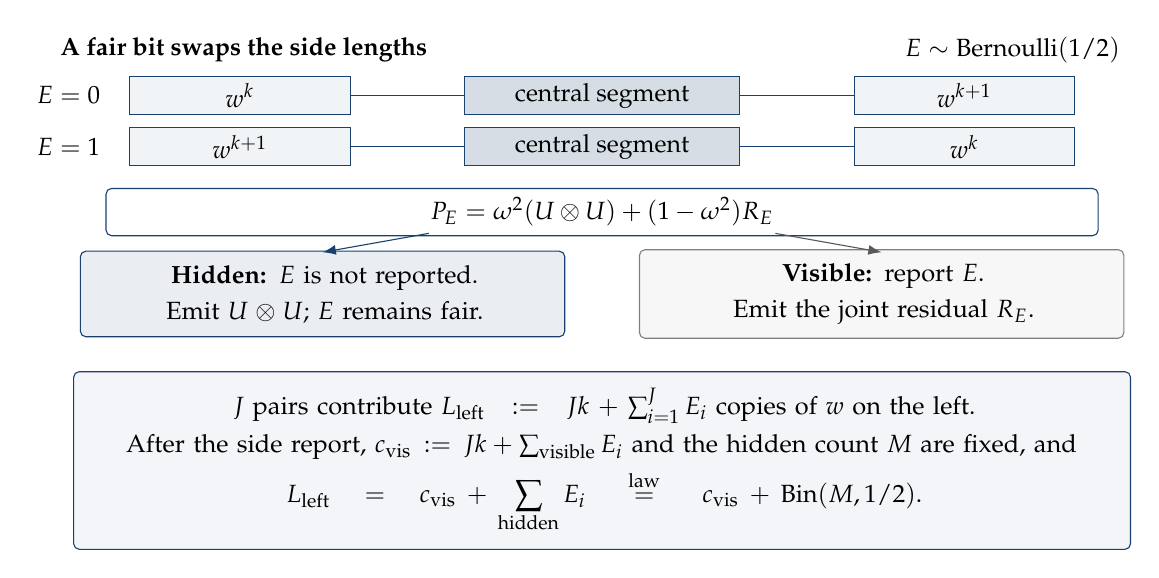
\begin{tikzpicture}[x=1cm,y=1cm,font=\small,>=Latex,
  side/.style={draw=linkblue,fill=linkblue!6,minimum width=2.8cm,
               minimum height=0.48cm,inner sep=2pt},
  center/.style={draw=linkblue,fill=linkblue!18,minimum width=3.5cm,
                 minimum height=0.48cm,inner sep=2pt},
  card/.style={draw=linkblue,rounded corners=2pt,align=center,
               text width=5.8cm,minimum height=0.94cm,inner sep=5pt}]
  \node[anchor=west,font=\small\bfseries] at (0,0.58)
    {A fair bit swaps the side lengths};
  \node[anchor=east] at (13.7,0.58)
    {$E\sim\mathrm{Bernoulli}(1/2)$};

  \node[anchor=east] at (0.75,0) {$E=0$};
  \node[side] at (2.4,0) {$w^k$};
  \node[center] at (7.0,0) {central segment};
  \node[side] at (11.6,0) {$w^{k+1}$};
  \draw[linkblue] (3.8,0)--(5.25,0);
  \draw[linkblue] (8.75,0)--(10.2,0);

  \node[anchor=east] at (0.75,-0.65) {$E=1$};
  \node[side] at (2.4,-0.65) {$w^{k+1}$};
  \node[center] at (7.0,-0.65) {central segment};
  \node[side] at (11.6,-0.65) {$w^k$};
  \draw[linkblue] (3.8,-0.65)--(5.25,-0.65);
  \draw[linkblue] (8.75,-0.65)--(10.2,-0.65);

  \node[draw=linkblue,fill=white,rounded corners=2pt,
        minimum width=12.6cm,minimum height=0.54cm] (law) at (7.0,-1.48)
    {$P_E=\omega^2(U\otimes U)+(1-\omega^2)R_E$};
  \node[card,fill=linkblue!9] (hidden) at (3.45,-2.52)
    {\textbf{Hidden:} \(E\) is not reported.\\[2pt]
     Emit \(U\otimes U\); \(E\) remains fair.};
  \node[card,draw=black!50,fill=black!3] (visible) at (10.55,-2.52)
    {\textbf{Visible:} report \(E\).\\[2pt]
     Emit the joint residual \(R_E\).};
  \draw[->,linkblue] (4.8,-1.75)--(3.45,-1.99);
  \draw[->,black!65] (9.2,-1.75)--(10.55,-1.99);

  \node[draw=linkblue,fill=linkblue!5,rounded corners=2pt,
        text width=13.0cm,align=center,inner sep=6pt,anchor=north] at (7.0,-3.50)
    {\(J\) pairs contribute
     \(L_{\rm left}:=Jk+\sum_{i=1}^{J}E_i\) copies of \(w\) on the left.\\[3pt]
     After the side report, \(c_{\rm vis}:=Jk+\sum_{\rm visible}E_i\)
     and the hidden count \(M\) are fixed, and\\[3pt]
     \(\displaystyle
       L_{\rm left}=c_{\rm vis}+\sum_{\rm hidden}E_i
          \ \overset{\mathrm{law}}{=}\ 
       c_{\rm vis}+\mathrm{Bin}(M,1/2).\)};
\end{tikzpicture}
\caption{Let \(\omega U\) be a common sublaw of the trace laws of
\(w^k\) and \(w^{k+1}\). For orientation \(E\), \(P_E\) is the product
of its two side laws and \(R_E\) is the normalized joint residual.
Across \(J\) independent pairs straddling the segment,
\(M\sim\mathrm{Bin}(J,\omega^2)\) before reporting. The lower panel
conditions on flags, side outputs, and visible bits; \(L_{\rm left}\)
counts only copies contributed by the left pair members. Other fixed
material adds a deterministic location offset. Block widths are schematic.}
\label{fig:paired-hiding}
\end{figure}


Throughout, unless window boundaries or additional payloads are
specified explicitly, report only one unseparated output
per segment/chunk/residual, plus flags and revealed orientation bits
as indicated (not original word boundaries internal to that output).
Given a word $w$ and a count $k$ with $\ov(\Tr(w^k),\Tr(w^{k+1}))\ge\omega$, choose a common sublaw $\omega U$.  Two chunks use a paired random bit orientation giving lengths
$(k,k+1)$ or $(k+1,k)$ even when far separated in the concatenation.
Use one joint flag of probability $\omega^2$ and output from
$U\otimes U$ on it, otherwise reveal the bit and generate the
two traces jointly from the normalized residual after subtracting
$\omega^2 U\otimes U$ from the product law for that orientation.
Marginalizing flags yields the requisite conditionally independent
pair traces given orientations. Conditional on the augmented
pair data, the bit remains fair on the hidden event. Independent
pairs thus carry independent hidden fair bits conditional on this
part of the report. All auxiliary schedules/flags are redrawn
independently for each trace.

\newpage
\subsection{Conditioning to obtain a small likelihood score}
Separating a typical region from a small exceptional mass is also used in Hellinger estimates for trace reconstruction \citep[arXiv v2, Section 2]{Chase2021Lower}.  The following version keeps the full moment and simulation-error budgets.

\begin{lemma}[Clipping with a common event]\label{lem:clipping}
Fix a level $0\le i\le D$ and its parameters from Section~\ref{sec:scales}.  Suppose preliminary oracle laws have common
``side'' metadata with law $Q_{\rm side}$, and conditional densities
$G_x,G_y$ over a conditional reference $Q$, possibly depending on
metadata.  Require $\int G_x\,dQ=\int G_y\,dQ=1$ for $Q_{\rm side}$-almost every metadata value.  Use $Q_{\rm side}Q$ as the joint reference. Suppose
on a typical metadata event of probability $\ge1-o(\Delta)$ we have
uniform estimates
\begin{equation}\label{eq:clipcond}
\|G_x-1\|_{r_i},\|G_y-1\|_{r_i}\le N_i^{-\rho},
\qquad \|G_y-G_x\|_{r_i}^2\le N_i^{-d_i-.01}
\end{equation}
in $L^{r_i}(Q)$, where $\rho\ge 2^{-4B-10}$.
Then conditioning each law on the event consisting of typical metadata and $G_x\ge1/2$ changes it in total variation by $o(\Delta)$.  The conditioned laws $\mu,\nu$ satisfy $\nu\ll\mu$ and
\[
 \|d\nu/d\mu-1\|_{L^{r_i}(\mu)}^2\le N_i^{-d_i}.
\]
All these conclusions hold uniformly over $0\le i\le D$.
\end{lemma}

\begin{proof}
Condition each preliminary law separately on the same joint event
$A_{\mathrm{keep}}$ consisting of typical metadata and $G_x\ge1/2$. Its complement has joint reference
measure on the typical part $\le(2N_i^{-\rho})^{r_i}$, hence bad
mass $o(\Delta)$ under each preliminary law by Cauchy--Schwarz,
the moment bound, and the common atypical mass. The conditioned
laws therefore change postprocessing by $o(\Delta)$ in total variation.
Because $G_x\ge1/2$ on the conditioning event $A_{\mathrm{keep}}$,
the new $y$-law is dominated by the new $x$-law and their likelihood
ratio on the latter support is $c' G_y/G_x$ with a scalar
$c'=1+o(\Delta)$. Also
\[
 \int_{\{G_x\ge1/2,\ \mathrm{typical}\}}
  \left|G_y/G_x-1\right|^{r_i} G_x\,d(Q_{\rm side}Q)
 \le 2^{r_i-1} N_i^{-(d_i+.01)r_i/2}.
\]
Under the conditioned $x$-law this yields
$\|G_y/G_x-1\|_{r_i}\le 3 N_i^{-(d_i+.01)/2}$ for all large $n$
by taking the $r_i$-th root (the conditioning probability is $1-o(\Delta)$).
Thus
$\|c'G_y/G_x-1\|_{r_i}\le
c' \|G_y/G_x-1\|_{r_i}+|c'-1|\le N_i^{-d_i/2}$
as desired for large $n$, since $\Delta\le N_i^{-100 d_D}$.
In this calculation and throughout, any $o(\Delta)$ masses claimed
from \eqref{eq:clipcond} follow uniformly using the definition of
$r_i$ and $\log N_i\to\infty$; no uniform lower bound on the
unconditioned ratio or density is needed. For Hellinger comparisons
of preliminary laws one can similarly use the squared density
difference times $2$ on $G_x\ge1/2$ and $G_x+G_y$ on its complement.

\end{proof}

\section{An initial pair at the working deletion rate}\label{sec:initial}

This section supplies the induction with a pair whose squared score decays as \(N_0^{-2.20}\) and whose repeated traces have enough common mass to hide later offsets. The initial words have one defect in each alternating period. A finite signed pattern moves some of these defects by one slot in opposite directions. We first describe an observation that forgets the original slot labels, then use its conditional rank probabilities for two purposes: obtaining common mass for pure runs and bounding the score of the signed pair.

\begin{proposition}[Initial pair]\label{prop:initial}
For the parameters of Section~\ref{sec:scales}, there is a choice of the common constants in Definition~\ref{def:invariant} with \(M_B=1\) for which a level-zero pair exists with simulation error \(E_0\le\Delta\). One may choose
\(\omega=\exp(-C_9\Lambda)\) for an absolute constant \(C_9\), and \(C>2\) with \(\log C=O(\Lambda)\).
\end{proposition}

\subsection{Words and the reported mark lists}

In this section \(C_*,c_*>0\) denote absolute constants whose values may change between estimates; constants indexed by \(r\) or \(s_0\) may depend on those fixed indices.

Put \(N=N_0\), \(\eta=.004\), and
\[
 m=\lfloor N^{1/2-\eta}\rfloor,\qquad
 K=\lfloor N^{1/2-2\eta}\rfloor,\qquad
 k=\lfloor\delta m\rfloor,
\]
\[
 J=\left\lfloor
       \frac{\lfloor N/(2m-1)\rfloor-K}{2k+1}
    \right\rfloor,\qquad
 P=J(2k+1)+K.
\]
Lemma~\ref{lem:scale-margins} gives \(\Lambda=o(\log N)\), hence
\(\delta^{-1}=N^{o(1)}\). In particular \(\delta^3m\to\infty\),
\(m\delta^2\to\infty\), and \(K,k+1\le m\) for all sufficiently large instances. The definitions then give
\[
 J\asymp\delta^{-1}N^{2\eta},\qquad J=o(K),\qquad
 P(2m-1)\in[N/2,N].
\]
For the last assertion, \(P\) differs from \(\lfloor N/(2m-1)\rfloor\) by fewer than \(2k+1\), so the omitted length is \(O(km+m)=o(N)\).

For this construction only, let the ordinary block be
\(\mathsf A=01\) and the defect block be \(\mathsf D=1\). For
\(b\in\{-1,0,1\}\), define the period
\[
 W_b=\mathsf A^{\lfloor m/2\rfloor+b-1}\,
       \mathsf D\,
       \mathsf A^{m-\lfloor m/2\rfloor-b}.
\]
It has \(m\) blocks, with the defect at block position
\(\lfloor m/2\rfloor+b\), and length \(2m-1\). Period, slot, and rank indices in this section start at \(1\). For even \(m\), the adjacent types \(W_0,W_1\) are exactly the shifted-defect pair displayed by \citet[arXiv v2, Introduction and Theorem~1]{Chase2021Lower}; for odd \(m\), they are the corresponding smaller pair with one common final \(\mathsf A\) appended. Below we compare \(W_{-1}\) with \(W_1\) in exceptional periods and make signed choices across many periods.

Set
\[
\begin{gathered}
 a=\lfloor P/2\rfloor,\qquad s_0=300,\qquad I=\{0,\ldots,2^{s_0}-1\},\\
 \sum_{i\in I}\beta_i z^i=\prod_{v=0}^{s_0-1}(1-z^{2^v}).
\end{gathered}
\]
The two words \(x_0,y_0\) have \(P\) periods. Every period is \(W_0\) except those at \(a+i\), \(i\in I\), where \(x_0\) uses \(W_{\beta_i}\) and \(y_0\) uses \(W_{-\beta_i}\). For all sufficiently large instances these indices lie in \(\{1,\ldots,P\}\). Both words have length
\(\ell_0=P(2m-1)\in[N/2,N]\), and they differ: the parse into \(01\) and \(1\) from the left is unique. The signs are the classical Prouhet--Thue--Morse signs; their polynomial has a zero of order \(s_0\) at \(1\) \citep[Proposition~2 and Theorem~6]{AlloucheShallit1999}.

We now define the more informative observation used only at this level. For \(H\in\{\mathsf A,\mathsf D\}\), put
\[
 r_e=\delta^2/2,\qquad
 \nu_H=\frac{\Tr(H)-r_e\delta_\varnothing}{1-r_e},
\]
where \(\varnothing\) denotes the empty string. This reserves the same empty output mass in both block laws. In the proof of Lemma~2.1, steps (I) and (III), \citet{HoldenLyons2020} first erase a mass \(q^2/2\) from \(01\) blocks at their deletion rate \(q\); here the same decomposition is applied at rate \(\delta\) to both \(01\) and \(1\), followed by an explicit likelihood score.

For each block independently, silently erase it with probability \(r_e\); otherwise report a mark with law \(\nu_H\). The mark alphabet is
\[
 \mathcal M_{\rm mark}=\{\varnothing,0,1,01\}.
\]
An observation on a sequence of blocks is the ordered list of its returning marks, an element of \(\bigsqcup_{l\ge0}\mathcal M_{\rm mark}^l\). The list reports its individual entries, including empty-valued entries, but no original slot labels or period boundaries. Thus the empty list and the one-entry list \((\varnothing)\) are distinct. Its count \(l\) is the number of entries, not the number of bits in their concatenation. Concatenating the mark strings gives the ordinary trace law, since
\(\Tr(H)=r_e\delta_\varnothing+(1-r_e)\nu_H\).

Under \(\nu_{\mathsf A}\), define
\[
 Z(Y)=\frac{\nu_{\mathsf D}(Y)}{\nu_{\mathsf A}(Y)}-1.
\]
The defect law is dominated by the ordinary-block law. Its support is contained in \(\{\varnothing,1\}\), where the likelihood ratios are
\[
 \frac{\delta-\delta^2/2}{\delta^2/2}
 \quad\text{and}\quad \frac1\delta,
\]
respectively. Hence \(Z\) is centered, \(\|Z\|_\infty=O(\delta^{-1})\), and
\(\|Z\|_{L^2(\nu_{\mathsf A})}^2\lesssim\delta^{-1}\), uniformly for \(\delta\le1/2\).

\subsection{Conditional densities and the rank kernel}

Consider \(1\le u\le m\) periods with fixed types
\(\mathbf b=(b_1,\ldots,b_u)\in\{-1,0,1\}^u\). There are \(n_b=um\) slots, and the defect in period \(j\) is at
\[
 p_{\mathbf b}(j)=(j-1)m+\lfloor m/2\rfloor+b_j.
\]
The return count has law \(\operatorname{Bin}(n_b,1-r_e)\), independent of \(\mathbf b\). Conditional on any count \(0\le l\le n_b\), the returning subset \(S_l\) is uniform among the size-\(l\) subsets of \(\{1,\ldots,n_b\}\). This subset is not reported. If \(p\in S_l\), let \(\operatorname{rk}_{S_l}(p)\) be its rank in the increasing order on \(S_l\). Put \(Q_l=\nu_{\mathsf A}^{\otimes l}\), with \(Q_0\) the point mass on the empty list.

Relative to \(Q_l\), the density of the reported list \(Y=(Y_1,\ldots,Y_l)\) is
\begin{equation}\label{eq:base-density}
 G_{\mathbf b}^{(u,l)}(Y)
 =\mathbb E_{S_l}
   \prod_{\{j:p_{\mathbf b}(j)\in S_l\}}
       \bigl(1+Z(Y_{\operatorname{rk}_{S_l}(p_{\mathbf b}(j))})\bigr).
\end{equation}
Empty products are \(1\), so this also defines the density at \(l=0\). It integrates to one because each \(1+Z\) has mean one under \(\nu_{\mathsf A}\). To expand it, for \(1\le r\le u\) take an increasing tagged tuple
\(\mathbf j=(j_1,\ldots,j_r)\) of periods and an increasing rank tuple
\(1\le v_1<\cdots<v_r\le l\). Write \(p_h=p_{\mathbf b}(j_h)\), and put
\begin{equation}\label{eq:base-rank-event}
\begin{split}
 W_{\mathbf j,\mathbf b}(v)
 &=\Prob\bigl\{
 p_h\in S_l,\ 
 \operatorname{rk}_{S_l}(p_h)=v_h
 \text{ for every }h
 \bigr\},\\
 A_{r,\mathbf b}(v)&=\sum_{1\le j_1<\cdots<j_r\le u}
                         W_{\mathbf j,\mathbf b}(v).
\end{split}
\end{equation}
The event in \(W_{\mathbf j,\mathbf b}\) imposes no restriction on untagged slots, including other defects. It is the joint probability of the tagged returns and ranks within the count conditioning, rather than a rank law conditioned again on all tags returning.
Expanding the product in \eqref{eq:base-density} now gives
\begin{equation}\label{eq:base-density-expansion}
 G_{\mathbf b}^{(u,l)}(Y)
 =1+\sum_{r=1}^{u}\ \sum_{1\le v_1<\cdots<v_r\le l}
       A_{r,\mathbf b}(v)\prod_{h=1}^r Z(Y_{v_h}).
\end{equation}

Define the slot gaps and rank gaps by
\[
\begin{aligned}
 (g_0,\ldots,g_r)
   &=(p_1-1,p_2-p_1-1,\ldots,p_r-p_{r-1}-1,n_b-p_r),\\
 (z_0,\ldots,z_r)
   &=(v_1-1,v_2-v_1-1,\ldots,v_r-v_{r-1}-1,l-v_r).
\end{aligned}
\]
Their sums are \(n_b-r\) and \(l-r\). Put \(\theta=l/n_b\) and
\(f_g(z)=\Prob\{\operatorname{Bin}(g,\theta)=z\}\). Counting returning untagged slots in each gap gives the exact kernel
\begin{equation}\label{eq:base-rank-kernel}
\begin{aligned}
 W_{\mathbf j,\mathbf b}(v)
 &=\frac{\prod_{i=0}^{r}\binom{g_i}{z_i}}{\binom{n_b}{l}}\\
 &=\frac{\theta^r}{f_{n_b}(l)}
       \prod_{i=0}^{r}f_{g_i}(z_i).
\end{aligned}
\end{equation}
We set \(f_g(z)=0\) outside \(z\in\{0,\ldots,g\}\). The last expression represents the same uniform subset by independent Bernoulli-\(\theta\) sampling conditioned on its total, including the degenerate laws at \(\theta=0,1\); it does not change the actual erasure rate \(r_e\).

For the rank estimates, call a count admissible when
\[
 \theta=\frac{l}{n_b}\in[1-\delta^2,1-\delta^2/4].
\]

For a tagged tuple define the coarse gaps
\[
 \gamma_0=j_1-\tfrac12,\qquad
 \gamma_i=j_{i+1}-j_i\ (1\le i<r),\qquad
 \gamma_r=u-j_r+\tfrac12.
\]
They sum to \(u\), and \(g_i=m\gamma_i+\alpha_i\) with
\(|\alpha_i|\le3\). The end coarse gaps are positive half-integers and the internal coarse gaps are positive integers. In particular \(g_i\gtrsim m\); at an admissible count, their expected binomial success and failure counts tend to infinity uniformly by \(m\delta^2\to\infty\).

\begin{lemma}[Rank-kernel square sum]\label{lem:base-kernel}
For the \(u\)-period construction and admissible count above, and every \(1\le r\le u\),
\begin{equation}\label{eq:abase}
 \|A_{r,\mathbf b}\|_{\ell^2}^2
 \le (C_3/\delta)^r(u/m)^{r/2}r^{-r/2},
\end{equation}
where \(\ell^2\) uses counting measure on increasing rank tuples and \(C_3\) is absolute, uniformly in the deterministic period types and the admissible count.
\end{lemma}

\begin{proof}
Fix \(u,l,\mathbf b\); all kernels in this proof therefore share \(\theta\) and \(f_{n_b}(l)\). In an inner product, both kernels use the same rank tuple \(v\), hence the same rank-gap vector \(z(v)\). The correspondence between increasing \(v\) and nonnegative \(z\) with sum \(l-r\) gives
\[
 \langle W_{\mathbf j,\mathbf b},W_{\mathbf j',\mathbf b}\rangle
 =\frac{\theta^{2r}}{f_{n_b}(l)^2}
   \sum_{\substack{z_i\ge0\\\sum_i z_i=l-r}}
       \prod_{i=0}^{r}f_{g_i}(z_i)f_{g_i'}(z_i).
\]
Choose a largest \(\gamma_e\) in the first tuple, breaking ties by the least index. Then \(g_e\gtrsim mu/(r+1)\). Solve the total constraint for \(z_e\), bound that factor by its supremum, and drop the constraints on the other coordinates:
\begin{equation}\label{eq:base-inner-product}
 \langle W_{\mathbf j,\mathbf b},W_{\mathbf j',\mathbf b}\rangle
 \le\frac{\theta^{2r}}{f_{n_b}(l)^2}
      \sup_z f_{g_e}(z)f_{g_e'}(z)
      \prod_{i\ne e}\sum_z f_{g_i}(z)f_{g_i'}(z).
\end{equation}
No multiplicity is introduced when \(z_e\) is solved.

Stirling's formula at the mean \(l=\theta n_b\) gives
\(f_{n_b}(l)^{-2}\lesssim\theta(1-\theta)n_b\lesssim\delta^2n_b\).
Also
\[
 \sup_z f_{g_e}(z)f_{g_e'}(z)\lesssim(\delta^2g_e)^{-1}.
\]
When \(g_e'\ge g_e/2\), this follows from the binomial maximum
\(O((\theta(1-\theta)g)^{-1/2})\) for each factor. When
\(g_e'<g_e/2\), the means differ by a fixed multiple of \(g_e\), so at every common argument one factor is a Hoeffding tail of size
\(\exp(-c_* g_e)\) \cite[Theorem~2]{Hoeffding1963}, which is smaller than the asserted bound. The product of this supremum and the inverse squared denominator is therefore \(O(r+1)\). The Stirling constants are absolute because every relevant expected success and failure count is at least a fixed multiple of \(m\delta^2\to\infty\).

For each free coordinate we use
\begin{equation}\label{eq:base-binomial-convolution}
 \sum_z f_g(z)f_{g'}(z)
 \le (C_{\rm rk}/\delta)g^{-1/2}
       \exp\!\left(-c_{\rm rk}\frac{(g-g')^2}{g+g'}\right)
\end{equation}
with absolute positive constants. To see this, regard the sum as the probability that the difference of two independent binomials is zero. Tilt their product law by \(e^{t\,\mathrm{difference}}\), with
\(t=-e_0(g-g')/(g+g')\) and a sufficiently small absolute \(e_0>0\).
The log moment is
\[
 \theta t(g-g')+O(t^2(g+g'))
 \le-c_{\rm rk}(g-g')^2/(g+g'),
\]
since \(\theta\ge1/2\). Under the tilt independence is preserved, the Bernoulli odds are multiplied by \(e^{\pm t}\), and the failure probabilities remain comparable to \(\delta^2\). The probability of zero under this tilted law is at most the first binomial's maximum mass \(O((\delta\sqrt g)^{-1})\), proving \eqref{eq:base-binomial-convolution}.

Corresponding coarse-gap coordinates have integer differences. Since
\(g_i=m\gamma_i+O(1)\) with an absolute error, for a nonzero mismatch and all large \(m\),
\[
 |g_i-g_i'|\ge\tfrac12m|\gamma_i-\gamma_i'|,
 \qquad g_i+g_i'\lesssim mu,\qquad g_i\gtrsim m\gamma_i.
\]
For a matching coordinate the exponential below is \(1\). Substituting these comparisons into \eqref{eq:base-inner-product} and using \(\theta^{2r}\le1\) yields the intermediate bound
\begin{equation}\label{eq:base-coarse-inner}
 \langle W_{\mathbf j,\mathbf b},W_{\mathbf j',\mathbf b}\rangle
 \le C_{\rm rk}(r+1)
 \prod_{i\ne e}\left[
   \frac{C_{\rm rk}}{\delta\sqrt{m\gamma_i}}\,
   \exp\!\left(-c_{\rm rk}
        \frac{m(\gamma_i-\gamma_i')^2}{u}\right)\right].
\end{equation}

It remains to sum this expression over both tagged tuples. Once the other coarse gaps are fixed, the constraint \(\sum_i\gamma_i=u\) determines the eliminated gap; the same holds for \(\gamma'\). For fixed \(\gamma\), dropping validity of the determined \(\gamma_e'\) can only enlarge the sum, and
\[
 \sum_{\gamma'}\prod_{i\ne e}
       e^{-c_{\rm rk}m(\gamma_i-\gamma_i')^2/u}
 \le\prod_{i\ne e}\sum_{z\in\mathbb Z}
       e^{-c_{\rm rk}(m/u)z^2}
 \le C_{\rm rk}^r
\]
because \(m\ge u\). Thus the remaining \(r\) first-tuple coordinates contribute \(m^{-r/2}\) times a sum of
\(\prod_{i\ne e}\gamma_i^{-1/2}\) with their total at most \(u\).
With \(\tau=r/u\in(0,1]\),
\[
 \sum_{\sum_{i\ne e}\gamma_i\le u}
       \prod_{i\ne e}\gamma_i^{-1/2}
 \le e^{\tau u}\prod_{i\ne e}
       \sum_{\gamma_i>0}\gamma_i^{-1/2}e^{-\tau\gamma_i}
 \le C_{\rm rk}^r(u/r)^{r/2}.
\]
The last lattice sum is \(O(\tau^{-1/2})\) on both the positive integer and positive half-integer lattices, by comparison with the integral of \(x^{-1/2}e^{-\tau x/2}\). Finally sum over the \(r+1\) possible selected coordinates \(e\). The resulting \(O((r+1)^2)\) factor is absorbed into a constant to the power \(r\). Since
\(\|A_{r,\mathbf b}\|_2^2\) is the sum of these inner products, this proves \eqref{eq:abase}.
\end{proof}

\subsection{Common mass for consecutive pure runs}

The rank estimate first gives common mass at the working deletion rate. This mass will later conceal the side orientations that move the exceptional periods as a group.

For \(u=k,k+1\), write \(G^{(u,l)}=G_{\mathbf0}^{(u,l)}\) for the conditional density of the list from \(W_0^u\). At a count \(l\) admissible for both totals, the two densities use the same \(Q_l\), although their respective parameters are \(\theta=l/(um)\). Orthogonality of distinct multilinear monomials in the independent centered scores gives
\[
 \mathbb E_{Q_l}\bigl[(G^{(u,l)})^2\bigr]
 =1+\sum_{r=1}^{u}\|A_{r,\mathbf0}\|_2^2\|Z\|_2^{2r}
 \le1+\sum_{r\ge1}
       (C_6\delta^{-2}\sqrt{u/m})^r r^{-r/2}
 \le\exp(C_6'\Lambda).
\]
Indeed, for \(a\ge0\),
\(\sum_{r\ge1}(a/\sqrt r)^r\le\exp(C_*(1+a^2))\): for \(r>4a^2\) the terms are at most \(2^{-r}\); for \(1\le r\le4a^2\), the maximum of \(r\log(a/\sqrt r)\) over positive reals is at most \(a^2/(2e)\). Here \(\delta^{-4}u/m\lesssim\delta^{-3}\) at both side counts.

Nonnegativity, mean one, and Cauchy--Schwarz imply
\[
 Q_l\{G^{(u,l)}\ge1/2\}\ge\tfrac14\exp(-C_6'\Lambda).
\]
Both densities are nondecreasing functions of the same coordinate likelihood values \(1+Z\ge0\): \eqref{eq:base-density} is an average of nonnegative products in those variables. The coordinates are independent under \(Q_l\). Increasing events for independent real coordinates are nonnegatively correlated, the independent-coordinate case of association \citep[Theorem~2.1]{EPW1967}. For completeness, in one dimension the covariance of increasing bounded functions \(f,g\) equals
\(\mathbb E[(f(X)-f(X'))(g(X)-g(X'))]/2\ge0\) for independent copies \(X,X'\). Induction conditions on the last coordinate and applies the same fact to the conditional means. Applying this to the two threshold events gives
\[
 \int\min(G^{(k,l)},G^{(k+1,l)})\,dQ_l
 \ge\tfrac1{32}\exp(-2C_6'\Lambda).
\]

The count laws overlap on
\[
 |l-(1-r_e)km|\le m.
\]
For either \(n_b=km\) or \(n_b=(k+1)m\), every such count is admissible for all large instances: its distance from the corresponding mean is at most \(2m\), and
\(m/n_b\asymp1/(\delta m)=o(\delta^2)\).
Stirling's formula gives mass per count at least
\[
 c_7(\delta\sqrt{n_b})^{-1}
       \exp\!\left(-C_7\frac{m^2}{\delta^2n_b}\right)
 \ge m^{-1}\exp(-C_8\Lambda)
\]
for absolute positive constants. One way to see the exponent is that the relative entropy between
\(\operatorname{Ber}(l/n_b)\) and \(\operatorname{Ber}(1-r_e)\) is at most a constant times
\((l/n_b-(1-r_e))^2/\delta^2\), while
\[
 (l/n_b)(1-l/n_b)n_b\asymp\delta^2n_b
 \asymp\delta^3m^2\longrightarrow\infty.
\]
There are at least \(m\) integer counts in this interval. Sum the conditional overlap bounds with the lesser of the two count probabilities. For a sufficiently large absolute \(C_9\), the mark-list laws of \(W_0^k,W_0^{k+1}\) have overlap at least
\[
 \omega=\exp(-C_9\Lambda)<1/8.
\]
Their ordinary trace laws have at least the same overlap by concatenation. Choose
\(C=\max\{C_{\rm abs}/\omega,9/\delta\}\). Then \(C\delta>8\) and \(\log C=O(\Lambda)\).

\subsection{The preliminary observation and its high-degree terms}

We use the common mass just obtained for the mark-list laws. Draw \(J\) independent fair bits \(E_1,\ldots,E_J\). Pair a run of \(k+E_i\) periods before a central run of \(K\) periods with a run of \(k+1-E_i\) periods after it; use a fixed order for the runs on each side. The number of periods before the central run is
\[
 L_{\rm left}=Jk+\sum_{i=1}^J E_i.
\]
For every schedule the exceptional global period \(a+i\) has central index \(X+i\), where
\begin{equation}\label{eq:base-anchor}
 X=a-L_{\rm left}
   =\left\lfloor\frac{J+K}{2}\right\rfloor-\sum_{i=1}^J E_i
   =K/2+O(J+1).
\end{equation}
Since \(J=o(K)\) and \(|I|\) is fixed, all exceptional periods lie in the central run for every schedule. Thus each schedule cuts the same prescribed word into pure side runs and a central run with the indicated translated types.

Use the paired flag construction of Section~\ref{sec:tools} on each pair of side mark-list laws, with a common sublaw \(\omega U\) on the list space. Report the flag and both lists; report the orientation bit only on the visible flag. Report one ordered list of individual marks from the central run, without period boundaries or original slot labels. The list values, including empty-valued entries, are retained. The full report also records the fixed left/right order of its side lists.

Let \(P_+,P_-\) be these preliminary report laws for \(x_0,y_0\), and let \(P_{\rm pure}\) be the corresponding law for \(W_0^P\). There is one deterministic projection \(\mathcal K_0\): discard the flags and bits and concatenate all mark values in chronological order. Conditional on any orientation schedule, averaging the pair flags gives independent correct side-list laws; the central list is generated independently from the actual central types. The schedule partitions the same word as just observed. Consequently
\begin{equation}\label{eq:base-exact-projection}
 \mathcal K_0P_+=\Tr(x_0),\qquad
 \mathcal K_0P_-=\Tr(y_0),\qquad
 \mathcal K_0P_{\rm pure}=\Tr(W_0^P).
\end{equation}

For the score analysis, the metadata consist of the side flags and lists, the visible bits, and the central list count \(l\); they exclude the central mark values. Their law \(Q_{\rm meta}\) is common to all three words. The count is independent of the side data and of \(X\), because the \(Km\) central erasures have the same probabilities for every type. Given a metadata value \(\mathfrak d\), let \(M\) be the number of hidden pairs. The remaining hidden bits are independent and fair, so the conditional law \(\pi_{\mathfrak d}\) of \(X\) is a constant minus \(\operatorname{Bin}(M,1/2)\).

Extend \(\beta_i\) by zero outside \(I\), and define the central type vectors by
\((\mathbf b_\pm(X))_j=\pm\beta_{j-X}\). Conditional on \(\mathfrak d\), the central densities and their coefficient arrays are
\begin{equation}\label{eq:base-central-mixture}
\begin{aligned}
 G_\pm^{\mathfrak d}
   &=\mathbb E_{X\sim\pi_{\mathfrak d}}G_{\mathbf b_\pm(X)}^{(K,l)},
 &A_{r,\pm}^{\mathfrak d}
   &=\mathbb E_{X\sim\pi_{\mathfrak d}}A_{r,\mathbf b_\pm(X)},\\
 G_{\rm pure}^{\mathfrak d}&=G_{\mathbf0}^{(K,l)},
 &A_{r,\rm pure}^{\mathfrak d}&=A_{r,\mathbf0}.
\end{aligned}
\end{equation}
These densities all integrate to one under \(Q_l\). In particular
\[
 P_\pm(d\mathfrak d,dY)
 =Q_{\rm meta}(d\mathfrak d)\,
       G_\pm^{\mathfrak d}(Y)Q_l(dY),
\]
with \(l\) read from \(\mathfrak d\), and the analogous identity holds for \(P_{\rm pure}\). This is the common conditional reference required by Lemma~\ref{lem:clipping}.

Call metadata typical when
\[
 \frac l{Km}\in[1-\delta^2,1-\delta^2/4],
 \qquad M\ge\omega^2J/2.
\]
The first failure is a multiplicative binomial tail for the central erasures, and the second is one for the independent hidden flags. The scale margins make both negligible at the required final-length budget:
\[
 (d_D+B+1)\log n=N^{o(\epsilon)},\qquad
 \delta^2Km=N^{1-3\eta-o(1)},\qquad
 \omega^2J=N^{2\eta-o(1)}.
\]
Thus both Chernoff exponents dominate
\(\log\Delta^{-1}=100(d_D+B+1)\log n\), and atypical metadata have mass \(o(\Delta)\).

Fix typical metadata for the remainder of the coefficient analysis and suppress the superscript \(\mathfrak d\). Put
\(\lambda=\sqrt{K/m}=N^{-\eta/2+o(1)}\).
For a fixed central type vector, Lemmas~\ref{lem:base-kernel} and~\ref{lem:moment} give
\[
 \left\|\sum_{1\le v_1<\cdots<v_r\le l}
      A_{r,\mathbf b}(v)\prod_{h=1}^r Z(Y_{v_h})\right\|_{r_0}
 \le \left(C_*r_0\delta^{-3/2}\sqrt\lambda\right)^r r^{-r/4}.
\]
Here \(\|Z\|_{r_0}\lesssim\delta^{-1}\), and
\(r_0,\delta^{-1}=N^{o(1)}\). The factor in parentheses is
\(N^{-\eta/4+o(1)}=N^{-.001+o(1)}\). Put \(R_0=3000\), and for each of the three densities write \(G_{\ge R_0}\) for the sum of its homogeneous terms of degrees at least \(R_0\) in \eqref{eq:base-density-expansion} and \eqref{eq:base-central-mixture}. Geometric summation, followed by Minkowski's inequality when mixing over \(X\), gives
\begin{equation}\label{eq:base-high-degrees}
\begin{aligned}
 \|G-1\|_{r_0}&\le N^{-.0009},\\
 \|G_{\ge R_0}\|_{r_0}&\le N^{-2.3}.
\end{aligned}
\end{equation}
The growing \(r_0\) is a moment order; \(R_0\) is a fixed degree cutoff. It remains to estimate the differences of their finitely many lower-degree arrays.

\subsection{Differences of one rank kernel}

For a tagged tuple in the central \(K\) periods, let \(W_{\mathbf j}\) be its type-\(W_0\) kernel. Let \(T_h\) move the \(h\)-th tagged slot one position to the right, while the rank tuple stays fixed, and put
\[
 D_h=(T_h-T_h^{-1})/2,\qquad
 V_h=(T_h+T_h^{-1}-2)/2.
\]
These operators change only the adjacent slot-gap lengths. In particular the total \(Km\), the count \(l\), the parameter \(\theta=l/(Km)\), and the denominator \(f_{Km}(l)\) remain fixed.

\begin{lemma}[Finite differences of a rank kernel]\label{lem:base-differences}
Fix \(1\le r<R_0\), an admissible central count, and a tagged tuple in \(K\) periods with coarse gaps \(\gamma_i\). For disjoint sets
\(\mathcal D,\mathcal V\subseteq\{1,\ldots,r\}\), put
\(v'=|\mathcal D|+2|\mathcal V|\). Then
\begin{equation}\label{eq:abase-diff}
 \left\|\prod_{h\in\mathcal D}D_h
             \prod_{h\in\mathcal V}V_h W_{\mathbf j}\right\|_{\ell^2}^2
 \le \delta^{-O_r(1)}\sqrt{Km}\,m^{-v'}
             \prod_{i=0}^r(m\gamma_i)^{-1/2}.
\end{equation}
The implicit constants depend only on \(r\).
\end{lemma}

\begin{proof}
Let \(S_i\) increase gap \(i\)'s length in the numerator of
\eqref{eq:base-rank-kernel}. Since \(T_h=S_{h-1}S_h^{-1}\),
\[
\begin{aligned}
 D_h&=\tfrac12(T_h-1)(1+T_h^{-1}),&
 V_h&=\tfrac12(T_h-1)^2T_h^{-1},\\
 T_h-1&=(S_{h-1}-1)S_h^{-1}+(S_h^{-1}-1).
\end{aligned}
\]
Use also \(S_i^{-1}-1=-(S_i-1)S_i^{-1}\). Expanding assigns exactly \(v'\) first length differences to gaps, with \(C_r\) terms and shifts of their lengths by \(O_r(1)\). For an assigned term write \(b_i\) for the order on gap \(i\); thus \(\sum_i b_i=v'\).

Write \((\nabla f)_g=f_{g+1}-f_g\) for the first length difference. At any integer length \(g\ge1\), the order-\(b\) difference \((\nabla^b f)_g\) has Fourier transform
\[
 \theta^b(e^{it}-1)^b(1-\theta+\theta e^{it})^g.
\]
On \([-\pi,\pi]\) the last factor has modulus at most
\(\exp(-c_*\delta^2g t^2)\), since \(\theta(1-\theta)\gtrsim\delta^2\).
Parseval and Fourier inversion therefore give, respectively,
\[
 \|(\nabla^b f)_g\|_2^2
 \le C_b\delta^{-(2b+1)}g^{-b-1/2},\qquad
 \|(\nabla^b f)_g\|_\infty^2
 \le C_b\delta^{-(2b+2)}g^{-b-1}.
\]
All shifted lengths are comparable to \(g_i\) for large \(m\), because \(r\) is fixed and \(g_i\gtrsim m\).

Choose a largest coarse gap \(e\), so its shifted length
\(\widetilde g_e\gtrsim_r Km\). In the squared rank sum, solve for \(z_e\) and use the squared supremum there, with squared \(\ell^2\) sums on the other \(r\) gaps. For one assigned term \(\mathcal F\), the displayed bounds and
\(f_{Km}(l)^{-2}\lesssim\delta^2Km\) give
\[
\begin{aligned}
 \|\mathcal F\|_2^2
 &\le C_r\delta^{-(2v'+r)}Km\,
       \widetilde g_e^{-1-b_e}
       \prod_{i\ne e}\widetilde g_i^{-1/2-b_i}\\
 &\le C_r\delta^{-(2v'+r)}
       \sqrt{Km}\,m^{-v'}
       \prod_{i=0}^r(m\gamma_i)^{-1/2}.
\end{aligned}
\]
The second line uses \(\widetilde g_i\gtrsim m\gamma_i\),
\(\widetilde g_i\gtrsim m\), and the extra factor
\(\widetilde g_e^{-1/2}\lesssim_r(Km)^{-1/2}\).
Combining the \(C_r\) assigned terms proves \eqref{eq:abase-diff}.
\end{proof}

\subsection{Signed coefficient arrays and their sums}

Define the seed motif indicator on the integers by
\(\chi_{\rm seed}(i)={\bf1}_{\{i\in I\}}\). The rank event depends on the type vector only through its tagged positions, so for a fixed \(X\),
\[
 W_{\mathbf j,\mathbf b_\pm(X)}
 =\prod_{h=1}^r T_h^{(\mathbf b_\pm(X))_{j_h}}W_{\mathbf j}.
\]
Each shift factor is exactly
\[
 T_h^{(\mathbf b_\pm(X))_{j_h}}
 =1+\chi_{\rm seed}(j_h-X)V_h
       \ \pm\ \beta_{j_h-X}D_h.
\]
For disjoint \(\mathcal D,\mathcal V\subseteq\{1,\ldots,r\}\), write
\[
 c_{\mathbf j}^{\mathcal D,\mathcal V}
 =\mathbb E_X\left[
       \prod_{h\in\mathcal D}\beta_{j_h-X}
       \prod_{h\in\mathcal V}\chi_{\rm seed}(j_h-X)\right],
 \qquad
 \partial_{\mathcal D,\mathcal V}
 =\prod_{h\in\mathcal D}D_h\prod_{h\in\mathcal V}V_h.
\]
The coefficient differences
\(B_r=A_{r,+}-A_{r,-}\) and
\(B_r^{\rm pure}=A_{r,+}-A_{r,\rm pure}\) come from
\eqref{eq:base-central-mixture}. Here and below, \(\sum_{\mathbf j}\) runs over \(1\le j_1<\cdots<j_r\le K\). Expanding the shift factors gives
\begin{equation}\label{eq:base-pattern-expansion}
 B_r
 =2\sum_{\substack{\mathcal D\cap\mathcal V=\varnothing\\
                    |\mathcal D|\ {\rm odd}}}
       \ \sum_{\mathbf j}
       c_{\mathbf j}^{\mathcal D,\mathcal V}
       \partial_{\mathcal D,\mathcal V}W_{\mathbf j}.
\end{equation}
For \(B_r^{\rm pure}\), the same expansion runs over all nonempty patterns, without the oddness restriction or the factor \(2\). These are finite sums of \(C_r\) patterns because \(r<R_0\) is fixed.

\paragraph{From individual tuples to the full array.}
Within the increasing rank tuples \(1\le v_1<\cdots<v_r\le l\), define
\[
 R_{\mathbf j}
 =\{v:|z_i(v)-\theta m\gamma_i|<m/8
           \text{ for }0\le i<r\}.
\]
These regions are disjoint. The first and internal coarse gaps determine the tuple, and any differing coordinate changes its center by at least \(\theta m\ge3m/4\), more than the combined radii \(m/4\). Bounded shifts of a kernel use the same region.

Fix one pattern and abbreviate its multiplier and operator by
\(c_{\mathbf j}\) and \(\partial\). Disjointness gives the weighted identity
\begin{equation}\label{eq:base-localized-array}
 \left\|\sum_{\mathbf j}{\bf1}_{R_{\mathbf j}}
                  c_{\mathbf j}\partial W_{\mathbf j}\right\|_2^2
 =\sum_{\mathbf j}|c_{\mathbf j}|^2
        \|{\bf1}_{R_{\mathbf j}}\partial W_{\mathbf j}\|_2^2
 \le\sum_{\mathbf j}|c_{\mathbf j}|^2
        \|\partial W_{\mathbf j}\|_2^2.
\end{equation}
The part outside these regions is negligible as an analytic coefficient estimate. To estimate it, expand \(D_h,V_h\) directly into tag shifts \(T_h\), which preserve the total \(Km\). Each resulting term is a fixed signed coefficient times a nonnegative shifted rank kernel. For each such kernel in \(\partial W_{\mathbf j}\), the conditional binomial formula and Hoeffding's inequality \cite[Theorem~2]{Hoeffding1963} give
\[
 \sum_{v\notin R_{\mathbf j}}W_{\mathbf j,\mathrm{shift}}(v)
 \le C_r f_{Km}(l)^{-1}e^{-c_* m/K}
 \le C_r\sqrt{Km}\,e^{-c_* m/K}.
\]
Indeed a bounded shift changes each relevant mean by \(O_r(1)\), while the excluded deviation is order \(m\), and each gap has length at most \(Km+O_r(1)\). Dropping the total constraint and taking a union bound over \(i<r\) proves the display. There are at most \(K^r\) tuples, the multiplier is bounded by \(1\), and \(\partial\) is a fixed linear combination of shifted kernels. Using \(\|\cdot\|_2\le\|\cdot\|_1\) for coefficient arrays, the discarded array has \(\ell^2\) norm at most
\[
 \tau_r=C_rK^r\sqrt{Km}\,e^{-c_* m/K}.
\]
It follows from \eqref{eq:base-localized-array} that the squared norm of the full array for this pattern is at most
\[
 2\sum_{\mathbf j}|c_{\mathbf j}|^2
        \|\partial W_{\mathbf j}\|_2^2+2\tau_r^2.
\]
This restriction does not condition a reported law or incur a total-variation error. Since \(m/K=N^{\eta+o(1)}\), even
\((C_*r_0\delta^{-1})^r\tau_r=o(N^{-A})\) for every fixed \(A\), uniformly over the finitely many \(r<R_0\).

\paragraph{Sums with one involved period fixed.}
The next two sums separate rank differentiation from the random location multiplier. For \(1\le h\le r\) and an integer \(j\), put
\[
 \Sigma_{r,h}(j)=\sqrt{Km}
 \sum_{\substack{1\le j_1<\cdots<j_r\le K\\j_h=j}}
             \prod_{i=0}^r(m\gamma_i)^{-1/2}.
\]
For \(r\ge2\), let \(\Sigma_{r,h}^{\rm bd}(j)\) be the same sum restricted to tuples with \(\gamma_i\le|I|\) for some \(1\le i<r\).

\begin{lemma}[Gap sums at a fixed period]\label{lem:base-fixed-sums}
For fixed \(1\le r<R_0\), uniformly in \(h\) and
\(j\in[K/3,2K/3]\),
\begin{equation}\label{eq:base-fixed-sums}
 \Sigma_{r,h}(j)\le C_r(Km)^{-1/2}\lambda^{r-1},\qquad
 \Sigma_{r,h}^{\rm bd}(j)
 \le C_{r,s_0}(Km)^{-1/2}m^{-1/2}\lambda^{r-2}\quad(r\ge2).
\end{equation}
\end{lemma}

\begin{proof}
The left gaps \(0,\ldots,h-1\) sum to \(j-\tfrac12\), and the right gaps \(h,\ldots,r\) sum to \(K-j+\tfrac12\). Each total is order \(K\). Select a largest gap on each side; both are at least \(c_rK\), so their two factors cost \(C_r(Km)^{-1}\). Given \(j\) and the other \(r-1\) gaps, the two total constraints determine the selected gaps. Each remaining free sum costs
\[
 \sum_{\substack{\gamma>0\\\gamma\le K}}(m\gamma)^{-1/2}
 \le C_*\sqrt{K/m}=C_*\lambda
\]
on either the integer or half-integer lattice. Grouping by the at most \(C_r\) choices of selected gaps and multiplying by \(\sqrt{Km}\) proves the first bound.

For the restricted sum, an internal gap at most \(|I|\) cannot be either selected largest gap for all sufficiently large \(K\). Union over its at most \(r-1\) possible indices. Its sum is at most
\(\sum_{\gamma=1}^{|I|}(m\gamma)^{-1/2}\le C_{s_0} m^{-1/2}\)
instead of \(C_*\lambda\). The other \(r-2\) free sums are unchanged, proving the second bound.
\end{proof}

\paragraph{The location multipliers.}
For the fixed metadata, \eqref{eq:base-anchor} shows that every
\(j\in\operatorname{supp}(\chi_{\rm seed}*\pi)\) satisfies
\(j=K/2+O(J+|I|)\), and hence lies in \([K/3,2K/3]\) for all large instances. Thus Lemma~\ref{lem:base-fixed-sums} applies to every involved period. For a sequence \(a\) on the integers, use the Fourier transform
\(\widehat a(t)=\sum_j a(j)e^{ijt}\). If \(M\ge\omega^2J/2\) is the hidden count, then
\[
 |\widehat\pi(t)|=|\cos(t/2)|^M\le e^{-c_*Mt^2}
 \qquad(-\pi\le t\le\pi).
\]
Since
\[
 \left|\sum_{i\in I}\beta_i e^{iti}\right|
 =\left|\prod_{v=0}^{s_0-1}(1-e^{i2^v t})\right|
 \le C_{s_0}|t|^{s_0},
\]
Parseval and the binomial decay give
\begin{equation}\label{eq:base-multiplier-norms}
\begin{aligned}
 \|\beta*\pi\|_2^2
 &\le C_{s_0} M^{-s_0-1/2}
 \le C_{s_0}\omega^{-2s_0-1}J^{-s_0-1/2},\\
 \|\chi_{\rm seed}*\pi\|_2^2
 &\le \|\chi_{\rm seed}\|_1^2\|\pi\|_2^2
 \le C_{s_0} M^{-1/2}
 \le C_{s_0}\omega^{-1}J^{-1/2}.
\end{aligned}
\end{equation}
The constants depending on \(s_0=300\) are fixed.

The dyadic signs turn convolution into a high-order finite difference. The same cancellation algebra appears in
\citet[Section~3.2, equation~(3.10)]{HMPW2008}, where iterated input-position differences act on a mean-coordinate binomial kernel. Here the signs are convolved with the conditional location law inside a likelihood coefficient; the terms involving several scores require the separate gap estimate above.

In \eqref{eq:base-pattern-expansion}, a singleton
\(\mathcal D=\{h\},\mathcal V=\varnothing\) has \(v'=1\) and multiplier
\((\beta*\pi)(j_h)\). Every other surviving pattern has an odd positive number of \(D\)'s, so \(v'\ge3\) and at least two indices are involved. At any chosen involved \(h\),
\[
 |c_{\mathbf j}^{\mathcal D,\mathcal V}|
 \le(\chi_{\rm seed}*\pi)(j_h).
\]
A nonzero multiplier requires all involved periods to lie in a common translate of \(I\). Two of them therefore differ by at most \(|I|-1\), so some intervening internal gap is at most \(|I|\).

For either kind of pattern choose such an involved \(h\), and let
\(\psi(j)\) be the corresponding envelope
\(|(\beta*\pi)(j)|\) or \((\chi_{\rm seed}*\pi)(j)\).
Apply Lemma~\ref{lem:base-differences} and first sum over tuples with \(j_h=j\):
\[
 \sum_{\mathbf j}|c_{\mathbf j}|^2
        \|\partial W_{\mathbf j}\|_2^2
 \le \delta^{-O_r(1)}m^{-v'}
       \sum_j\psi(j)^2
       \begin{cases}
          \Sigma_{r,h}(j),&\text{for a singleton},\\
          \Sigma_{r,h}^{\rm bd}(j),&\text{otherwise}.
       \end{cases}
\]
Now \eqref{eq:base-fixed-sums} and \eqref{eq:base-multiplier-norms} apply. Combining the finitely many patterns in
\eqref{eq:base-pattern-expansion} and the analytic tail gives
\begin{equation}\label{eq:base-low-coefficients}
\begin{aligned}
 \|B_r\|_2^2\le C_{r,s_0}\delta^{-O_r(1)}\Big[
 &\omega^{-2s_0-1}J^{-s_0-1/2}m^{-1}(Km)^{-1/2}\lambda^{r-1}\\
 &+{\bf1}_{r\ge2}\,\omega^{-1}J^{-1/2}
           (Km)^{-1/2}m^{-7/2}\lambda^{r-2}\Big]+C_r\tau_r^2.
\end{aligned}
\end{equation}
The nonlinear \(m^{-7/2}\) is \(m^{-3}\) from its minimum difference order and \(m^{-1/2}\) from the bounded internal gap. For \(B_r^{\rm pure}\), the singleton \(D\) contribution is the same. Every other pattern has \(v'\ge2\), but a singleton \(V\) requires no bounded internal gap. The full pure-comparison array therefore satisfies
\begin{equation}\label{eq:base-pure-coefficients}
\begin{aligned}
 \|B_r^{\rm pure}\|_2^2\le C_{r,s_0}\delta^{-O_r(1)}\Big[
 &\omega^{-2s_0-1}J^{-s_0-1/2}m^{-1}(Km)^{-1/2}\lambda^{r-1}\\
 &+\omega^{-1}J^{-1/2}
       (Km)^{-1/2}m^{-2}\lambda^{r-1}\Big]+C_r\tau_r^2.
\end{aligned}
\end{equation}

\subsection{Closing the initial invariant}

For each fixed \(r<R_0\), Lemma~\ref{lem:moment} converts the coefficient estimate to the required score estimate:
\[
 \left\|\sum_{1\le v_1<\cdots<v_r\le l}
       B_r(v)\prod_{h=1}^r Z(Y_{v_h})\right\|_{r_0}^2
 \le (C_1r_0\|Z\|_{r_0})^{2r}\|B_r\|_2^2.
\]
The analogous inequality applies to the pure comparison. The fixed pattern constants, the displayed powers of \(\delta^{-1}\) and \(\omega^{-1}\), and the moment factors are \(N^{o(1)}\): use
\(\log r_0=O_B(D+1)\), \(\log\omega^{-1}=O(\Lambda)\), and
\(\Lambda=o(\log N)\). The analytic tails remain below every fixed power after these factors.

The worst nonlinear term of \eqref{eq:base-low-coefficients}, at \(r=2\), is
\[
 J^{-1/2}(Km)^{-1/2}m^{-7/2}
 =N^{-\eta}\,N^{-1/2+3\eta/2}\,
       N^{-7/4+7\eta/2+o(1)}
 =N^{-9/4+4\eta+o(1)}=N^{-2.234+o(1)}.
\]
The singleton term is \(N^{-3.394+o(1)}\) at its worst degree \(r=1\). The worst nonlinear term in \eqref{eq:base-pure-coefficients} is
\(N^{-3/2+5\eta/2+o(1)}=N^{-1.49+o(1)}\).
Sum over the finitely many lower degrees and add the degree tails in \eqref{eq:base-high-degrees}. On every typical metadata value this yields
\begin{equation}\label{eq:base-score-differences}
 \|G_+-G_-\|_{r_0}^2\le N^{-2.22},\qquad
 \|G_+-G_{\rm pure}\|_{r_0}^2\le N^{-1.4}.
\end{equation}

Let \(\mathcal A\) be the joint event of typical metadata and
\(G_+^{\mathfrak d}(Y)\ge1/2\), and define
\[
 \mu_0=P_+(\,\cdot\mid\mathcal A),\qquad
 \nu_0=P_-(\,\cdot\mid\mathcal A).
\]
Lemma~\ref{lem:clipping} applies to the common conditional reference above: \eqref{eq:base-high-degrees} gives
\(\rho=.0009\ge2^{-4B-10}\), and \(2.22>2.20+.01\) supplies its difference margin. Hence
\[
 \nu_0\ll\mu_0,\qquad
 \|d\nu_0/d\mu_0-1\|_{L^{r_0}(\mu_0)}^2\le N^{-2.20},
\]
and conditioning changes each preliminary law by \(o(\Delta)\) in total variation. By \eqref{eq:base-exact-projection} and contraction under the same \(\mathcal K_0\),
\[
 \TV(\mathcal K_0\mu_0,\Tr(x_0))\le o(\Delta)\le\Delta,\qquad
 \TV(\mathcal K_0\nu_0,\Tr(y_0))\le o(\Delta)\le\Delta
\]
for all large instances. This gives \(E_0\le\Delta\) and the score part of the invariant. The hidden-bit law was used for the preliminary densities only.

It remains to transfer pure-run overlap to \(x_0\). This comparison uses the preliminary laws, rather than the full clipping conclusion for their weaker \(N^{-1.4}\) difference. On typical metadata and \(G_+\ge1/2\),
\[
 (\sqrt{G_+}-\sqrt{G_{\rm pure}})^2
 \le 2|G_+-G_{\rm pure}|^2.
\]
On the complement use the bound \(G_++G_{\rm pure}\). The high-moment estimate \eqref{eq:base-high-degrees} and the clipping proof bound the mass of the bad-density region under both preliminary laws by \(o(\Delta)\); atypical metadata have the same bound. Thus \eqref{eq:base-score-differences} gives
\[
 H^2(P_+,P_{\rm pure})\le2N^{-1.4}+o(\Delta)\le3N^{-1.4}.
\]
Projection by \(\mathcal K_0\) gives the same upper bound for
\(H^2(\Tr(x_0),\Tr(W_0^P))\).

Set \(k_0=\lceil CkP\rceil\). Since \(k\sim\delta m\) and
\(C\delta>8\), we have \(k_0\ge\ell_0\) for all large instances. Also,
\[
 \frac{k_0}{\ell_0}
 \le\frac{C\delta m}{2m-1}+\frac1{\ell_0}<C,
\]
using \(\delta\le1/2\), \(C\ge18\), and \(\ell_0\to\infty\). Thus the common choice \(M_B=1\) meets the level-zero count predicate. Moreover
\(C=\exp(O(\Lambda))=N^{o(1)}\). For \(F=k_0,k_0+1\), tensorization followed by concatenation therefore gives
\[
 \TV(\Tr(x_0^F),\Tr(W_0^{PF}))
 \le\sqrt{F\,H^2(\Tr(x_0),\Tr(W_0^P))}
 \le\sqrt{3F N^{-1.4}}
 =N^{-0.2+o(1)}=o(1).
\]
Lemma~\ref{lem:lift}, with base word \(W_0\), overlap count \(k\), replication \(P\), and \(F=k_0\), gives overlap at least \(2/3\) for the two pure repeated comparison words. Paying the two replacement costs leaves
\[
 \ov(\Tr(x_0^{k_0}),\Tr(x_0^{k_0+1}))
 \ge2/3-o(1)\ge\omega.
\]
Together with the length, distinction, score, and simulation estimates already proved, this completes Proposition~\ref{prop:initial}.

\section{One amplification block: words and overlap}\label{sec:block}

We now construct one longer pair from the preceding oracle pair.  This section defines the nested words and proves the consecutive-power overlap needed for their side runs.  Section~\ref{sec:layout} constructs the observation of those words, and Section~\ref{sec:coefficients} proves its score estimate.

\begin{proposition}[One amplification block]\label{prop:block}
For the parameters of Section~\ref{sec:scales}, let $1\le i\le D$ and suppose a level-$(i-1)$ pair satisfies Definition~\ref{def:invariant} with constants $C,\omega,M_B$.  Set
\[
 C'=\max\{C,C_{\rm abs}/\omega\}.
\]
The input pair remains valid when $C$ is replaced by $C'$, and there exists a level-$i$ pair satisfying the definition with the same constants $C',\omega,M_B$, with
\[
 d_i=d_{i-1}+(b_i-1)/4-.05,
 \qquad E_i\le\Delta+(\ell_i/\ell_{i-1})E_{i-1}.
\]
Every preceding level constructed with $C$ also remains valid with $C'$, and this enlarged value is retained in later blocks.  The conclusion is uniform over all levels along the stated joint asymptotic regime.
\end{proposition}

Fix $i$ for the proof.  The value $C'$ meets the hypothesis of Lemma~\ref{lem:lift}.  Every preceding upper count bound remains true after replacing $C$ by $C'$, since its exponent $2Bh+M_B$ at a level $h\ge0$ is nonnegative; the lower count bounds, scores, and projection errors do not involve $C$.  The enlarged constant still depends only on $\delta$ and satisfies $\log C'=O(\Lambda)$.  We henceforth write $C$ for $C'$ and use this common enlarged constant in the counts constructed below and in later blocks.

Abbreviate
\[
\begin{gathered}
 b=b_i,\quad N=N_i,\quad d=d_{i-1},\quad d'=d_i,\\
 x=x_{i-1},\quad y=y_{i-1},\quad \ell=\ell_{i-1},\quad k=k_{i-1}.
\end{gathered}
\]
Within this block write $a_0=a_0(b)$ for the contraction exponent defined in \eqref{eq:contraction-exponent}.  Thus $\ell\in[N^{a_0}/2,N^{a_0}]$.  Since $r_i\le r_{i-1}$, the old score satisfies
\begin{equation}\label{eq:old-score}
 \left\|\frac{d\nu_{i-1}}{d\mu_{i-1}}-1\right\|_{L^{r_i}(\mu_{i-1})}^2
       \le N^{-a_0d}.
\end{equation}

\subsection{Nested signed words}

The two new words will use the same nested motif at $b$ depths.  Choose the fixed degree cutoff and the cancellation order
\[
 r_*=2^{10B+40},\qquad
 s_*=\left\lceil100(d_D+r_*+B+10)/\epsilon\right\rceil,
 \qquad L=2^{s_*}.
\]
Let $\mathcal I=\{0,\ldots,L-1\}$ and define the signs by
\[
 \sum_{a\in\mathcal I}\sigma_a z^a
       =\prod_{v=0}^{s_*-1}(1-z^{2^v}).
\]
Extend $\sigma_a$ by zero outside $\mathcal I$, and put $\chi={\bf1}_{\mathcal I}$.  The order $s_*=O_B((D+1)^2)$ is large enough for the signed smoothing below at every block.  Lemma~\ref{lem:scale-margins} gives, uniformly,
\begin{equation}\label{eq:block-losses}
\begin{gathered}
 L^{O_B(r_*B)}=N^{o(\epsilon)},\\
 \exp\bigl(O_B((s_*+1)^2+(s_*+1)(D+1)\Lambda)\bigr)
       =N^{o(\epsilon)}.
\end{gathered}
\end{equation}
Here and below fixed-depth constants may depend on $B$.

Start with $U_0^+=x$, $U_0^-=y$, both of length $S_0=\ell$, and with overlap count $h_0=k$.  Once a positive integer $P_j$ has been chosen, form $U_j^\tau$, for $\tau\in\{+1,-1\}$, from $P_j$ consecutive level-$(j-1)$ atoms.  Use type $+$ except at the labels
$\lfloor P_j/2\rfloor+a$, $a\in\mathcal I$, where the type is $\tau\sigma_a$.  We choose the counts below so that these labels lie in $[1,P_j]$.  The common length is
\[
 S_j=P_jS_{j-1}.
\]
The two words are distinct: at a motif label their atom types differ, and equal-length atoms give a fixed parse back to the distinct old words.

\subsection{Word sizes, windows, and paired counts}

Write $N^{a_j}$ for the target length of a level-$j$ word.  It then contains about $N^{a_j-a_{j-1}}$ lower atoms.  An overlap chunk will contain $h_{j-1}$ such atoms, with $h_{j-1}$ within the controlled channel factor of their word length $N^{a_{j-1}}$.  To leave about $N^\epsilon$ paired chunks, choose the remaining exponents by
\[
 a_j(b)=2a_{j-1}(b)+\epsilon\quad(1\le j\le b).
\]
This recurrence and \eqref{eq:contraction-exponent} give the identities
\begin{equation}\label{eq:local-exponents}
 a_j(b)=(1+\epsilon)2^{j-b}-\epsilon\quad(0\le j\le b),
 \qquad a_b(b)=1.
\end{equation}
In the rest of this block, $a_j$ abbreviates $a_j(b)$.

A level-$j$ child window will contain $T_j$ level-$(j-1)$ atoms.  Define
\[
 \kappa_j=a_{j-1}-3(2^j-1)\epsilon,
 \qquad T_j=4\left\lfloor N^{\kappa_j}/4\right\rfloor
       \quad(1\le j\le b).
\]
The $\kappa_j$ are positive for all sufficiently large instances, uniformly in the block.  Directly from \eqref{eq:local-exponents},
\begin{equation}\label{eq:kj}
\begin{aligned}
 2\kappa_j-\kappa_{j+1}-\epsilon&=\epsilon\quad(1\le j<b),\\
 \kappa_b&>\epsilon,\qquad
 \kappa_j<a_{j-1}<a_j-a_{j-1}\quad(1\le j\le b).
\end{aligned}
\end{equation}
The first identity makes $T_j$ larger than the typical displacement from $T_{j+1}$ collections of about $N^\epsilon$ fair bits: the squared window width divided by that bit count has order $N^\epsilon$.  The remaining inequalities leave room for the windows inside their words.  We also have
\begin{equation}\label{eq:power_gap}
 \sum_{j=1}^b\kappa_j<1,
\end{equation}
since $\kappa_j<a_{j-1}<2^{j-1-b}$; this will bound the number of vertices in the observation tree.

For $1\le j<b$, choose
\[
\begin{aligned}
 P_j&=\left\lfloor N^{a_j}/S_{j-1}\right\rfloor,
 &h_j&=\lceil C h_{j-1}P_j\rceil,\\
 t_j&=2\left\lfloor P_j/[100(2h_{j-1}+1)]\right\rfloor.
\end{aligned}
\]
For the root, choose
\[
\begin{aligned}
 J&=\left\lfloor\frac{\lfloor N/S_{b-1}\rfloor-T_b}
                         {2h_{b-1}+1}\right\rfloor,
 &P_b&=J(2h_{b-1}+1)+T_b,\\
 h_b&=\lceil C h_{b-1}P_b\rceil.
\end{aligned}
\]
The counts $t_j$ and $J$ are the numbers of paired chunks used for local and outer displacements, respectively.  The factors $2$ and $4$ in their definitions and in $T_j$ ensure the parity and divisibility needed by the partition.

We record the size consequences before using the words.  For $j<b$, flooring loses at most $S_{j-1}=o(N^{a_j})$, so
\[
 S_j\in[N^{a_j}/2,N^{a_j}],\qquad
 P_j\asymp N^{a_j-a_{j-1}},\qquad T_j=o(P_j).
\]
The overlap counts remain within the declared uniform bound.  Indeed $h_j\ge S_j$ by induction, and
\[
 \frac{h_j}{S_j}\le C\frac{h_{j-1}}{S_{j-1}}+1
       \le C^2\frac{h_{j-1}}{S_{j-1}}
\]
because $h_{j-1}/S_{j-1}\ge1$ and $C>2$.  Starting from the level-$(i-1)$ bound gives
\begin{equation}\label{eq:nested-counts}
 S_j\le h_j\le C^{2B(i-1)+M_B+2j}S_j
             \le C^{2Bi+M_B}S_j\quad(0\le j\le b),
\end{equation}
In particular the extra count factor is at most $\exp(O_B((D+1)\Lambda))$.

Using these bounds in the definitions of $t_j$ and $J$ yields
\begin{equation}\label{eq:scale_t}
 e^{-O_B((D+1)\Lambda)}N^\epsilon\le t_j\le O(N^\epsilon)
       \quad(1\le j<b),
\end{equation}
and the same lower and upper bounds for $J$.  All these counts tend to infinity uniformly.  At the root, $J=o(T_b)$ by $\kappa_b>\epsilon$, and
\[
 N-S_b=O((h_{b-1}+1)S_{b-1})
 \le N^{2a_{b-1}+o(\epsilon)}
 =N^{1-\epsilon+o(\epsilon)}=o(N).
\]
Here the count overhead is $N^{o(\epsilon)}$ by \eqref{eq:uniform-absorption}, and $2a_{b-1}=1-\epsilon$ by \eqref{eq:local-exponents}.  Thus also $S_b\in[N/2,N]$.  Working backward from $\kappa_b>\epsilon$ in \eqref{eq:kj} gives $\kappa_j>\epsilon$ at every depth.  The uniform loss bound \eqref{eq:block-losses} therefore gives $L=o(T_j)$ and $L=o(P_j)$ uniformly, so all motif labels used above fit.  We take
\[
 x_i=U_b^+,\qquad y_i=U_b^-,\qquad \ell_i=S_b,\qquad k_i=h_b.
\]

The following estimate quantifies the smoothing supplied by a hidden binomial offset.  It will be used in the early overlap comparison and in the main score proof.  In those applications, its local parameter $m$ is one of the paired counts $J$ or $t_j$, while $g$ is the actual number of hidden orientation trials.
\begin{lemma}[Signed binomial smoothing]\label{lem:binomial-smoothing}
Let $\sigma$ be the Prouhet--Thue--Morse sequence of order $s_*$ above.  Suppose $\pi$ is an integer translation or reflection of a fair binomial probability mass function with $g\ge c_0\omega^2m$ trials, where $c_0>0$ is absolute and $m\to\infty$ as in the construction.  Then
\begin{align}
 \|\sigma*\pi\|_\infty
 &\le \exp(O((s_*+1)^2+(s_*+1)\Lambda))\,
       m^{-(s_*+1)/2},\nonumber\\
 \|\sigma*\pi\|_2^2
 &\le \exp(O((s_*+1)^2+(s_*+1)\Lambda))\,
       m^{-s_*-1/2},\qquad
 \|\pi\|_\infty\le O(\omega^{-1}m^{-1/2}).\label{eq:sig_conv}
\end{align}
The norms use counting measure on the integers, and the implicit constants may depend on $c_0$.
\end{lemma}

\begin{proof}
Translations and reflections do not affect the estimates.  For the first two, use Fourier inversion and Parseval.  On $[-\pi,\pi]$ the sign transform has modulus at most $2^{s_*(s_*-1)/2}|z|^{s_*}$, and the binomial transform has modulus at most $e^{-cgz^2}$.  Gaussian integration contributes, besides the power of $g$, a factor $\exp(O((s_*+1)\log(s_*+1)))$.  The last estimate is the binomial maximum bound from Stirling's formula.
\end{proof}

\subsection{Overlap for each nested atom}\label{sec:side-overlap}

\begin{lemma}[Overlap of the nested atoms]\label{lem:nested-overlap}
Under the input hypotheses of Proposition~\ref{prop:block}, the words and counts constructed above satisfy, for every $1\le j\le b$,
\[
 \ov\bigl(\Tr((U_j^+)^{h_j}),\Tr((U_j^+)^{h_j+1})\bigr)\ge\omega.
\]
\end{lemma}

\begin{proof}
The old score and the two projection errors give
\begin{equation}\label{eq:old_H}
 H^2(\Tr(x),\Tr(y))\le O(N^{-a_0d}+E_{i-1}).
\end{equation}
Indeed the score bounds the squared Hellinger distance of the old oracle laws, and contraction followed by the Hellinger triangle inequality handles the two projection errors.

For the induction on $j$, assume the overlap statement at level $j-1$; at $j=1$ it is the input invariant.  Lemma~\ref{lem:lift}, with base word $U_{j-1}^+$, overlap count $h_{j-1}$, replication $P_j$, and $F=h_j\ge C h_{j-1}P_j$, gives overlap at least $2/3$ for the two pure comparison words formed by repeating $P_j$ copies of $U_{j-1}^+$.  Replacing one such length-$S_j$ unit by $U_j^+$ changes at most $L$ lower atoms.  For $h_j$ or $h_j+1$ repeated units, the squared Hellinger replacement cost is therefore at most
\begin{equation}\label{eq:nested-replacement}
 (h_j+1)L\,H^2(\Tr(U_{j-1}^+),\Tr(U_{j-1}^-)).
\end{equation}

The two phases of the depth schedule give the margins needed here.  From \eqref{eq:local-exponents} and the choice of $\epsilon$, for $b=2$ and $d\ge2.20$,
\begin{equation}\label{eq:b2gap}
 a_0d-a_1>.03,\qquad 2a_0d>1.06.
\end{equation}
For $i>j_0$, we have $b=B$ and $d\ge2^B+2.20$, giving
\begin{equation}\label{eq:bbgap}
 a_0d>1+2^{-B}.
\end{equation}
For example, before the $\epsilon d$ correction the first two left sides are at least $.05$ and $1.10$, and the last is at least $1+2.20\,2^{-B}$.  The bound $d\le2.20+(B/4)D$ and $\epsilon=2^{-4B-100}/(D+1)$ leave the displayed margins uniformly.

In a block with $i>j_0$, the two level-$(j-1)$ atoms differ on at most $L^{j-1}$ old atoms.  Tensorization, concatenation, and \eqref{eq:old_H} therefore bound \eqref{eq:nested-replacement} by $o(1)$: use \eqref{eq:bbgap}, $h_j\le e^{O_B((D+1)\Lambda)}N$, $L^b=N^{o(\epsilon)}$, and $E_{i-1}\le n(D+1)\Delta$.  In a preliminary block, $b=2$.  At $j=1$ the same argument uses $h_1\le e^{O_B((D+1)\Lambda)}N^{a_1}$ and the first inequality in \eqref{eq:b2gap}.  At $j=2$ we need the sharper comparison
\begin{equation}\label{eq:side_refine}
 H^2(\Tr(U_1^+),\Tr(U_1^-))
 \le N^{-2a_0d+o(\epsilon)}+O(P_1E_{i-1}+\Delta),\qquad b=2.
\end{equation}
The second inequality in \eqref{eq:b2gap} then makes \eqref{eq:nested-replacement} $o(1)$ at the root as well.

To prove \eqref{eq:side_refine}, report a single window of $T_1$ separate old oracle outputs.  Its nominal start is after
$A=\lfloor(P_1-T_1)/2\rfloor$ old atoms.  Put $t_1$ paired pure-$x$ chunks before and after the window, with counts $h_0+E,h_0+1-E$ for independent fair bits $E$.  Use the paired flag construction at the input overlap.  Complete the two sides by pure-$x$ residuals of counts
\[
 A-t_1(h_0+1/2),\qquad P_1-T_1-A-t_1(h_0+1/2).
\]
These are nonnegative integers.  Chunks and residuals have fixed relative IDs and each reports one unseparated ordinary trace, together with its flag and any revealed bit.  The window start displacement $V$ is the sum of the $t_1$ bits minus $t_1/2$, so $|V|\le t_1/2=o(T_1)$.  Every motif label therefore lies in the window.

Conditional on the orientation bits, sample the $T_1$ window outputs independently of one another and of the entire collection of side flags and emissions, using $\mu_{i-1}$ for an $x$ atom and $\nu_{i-1}$ for a $y$ atom at the corresponding rank.  Inside the window, report the old oracle outputs with their relative ranks, but not their absolute start or type labels.  Apply $\mathcal K_{i-1}$ independently to these outputs and concatenate in the scheduled order.  Given the orientation bits, averaging the flags produces the exact independent trace laws of the other pieces.  The common projection therefore approximates the genuine trace with error at most $T_1E_{i-1}$ under either hypothesis.

Except on side metadata of probability $o(\Delta)$, at least $\omega^2t_1/2$ orientations are hidden, by binomial concentration and \eqref{eq:scale_t}.  Conditional on such metadata, $V$ is a translated fair binomial with that many trials.  Relative to $Q=\mu_{i-1}^{\otimes T_1}$, let $G_+,G_-$ be the conditional densities of the window outputs.  For fixed $V$, each is a product of at most $L$ factors $1+Z$ at distinct positions, averaged over $V$, where $Z$ is the old score.  Lemma~\ref{lem:moment} gives for its homogeneous degree-$r$ part the squared $L^{r_i}(Q)$ bound
\[
 (C_1r_i)^{2r}N^{-a_0dr}\binom Lr.
\]
Convexity permits averaging over $V$ at the same bound.  Geometric summation gives
\[
 \|G_\pm-1\|_{r_i}\le N^{-a_0d/2+o(\epsilon)},
\]
and the squared norm of the terms of degree at least two is at most $N^{-2a_0d+o(\epsilon)}$.  In $G_+-G_-$ the singleton coefficient array is, up to signs, the convolution of $\sigma$ with the law of $V$.  Equation~\eqref{eq:sig_conv} and \eqref{eq:scale_t} bound its square sum strongly enough that
\[
 \|G_+-G_-\|_{r_i}^2\le N^{-2a_0d+o(\epsilon)};
\]
indeed $t_1^{-s_*}\le N^{-\epsilon s_*}
\exp(O_B((D+1)s_*\Lambda))$.

On typical metadata, the region $G_+<1/2$ has mass $o(\Delta)$ under both laws by the same moment argument as in Lemma~\ref{lem:clipping}.  On its complement, the squared density difference bounds Hellinger distance.  Adding the atypical metadata and projection errors proves \eqref{eq:side_refine}, with fixed numerical factors absorbed in $o(\epsilon)$.  Thus all replacement costs in \eqref{eq:nested-replacement} are $o(1)$.  The pure overlap $2/3$ loses at most the two replacement total variations, and remains above $\omega<1/8$.  This completes the overlap induction.
\end{proof}

The words, counts, and overlaps required for the observation are now available at every nested depth.  The next section uses their paired side runs to hide the relative locations of the motifs.

\section{An observation with randomly displaced windows}\label{sec:layout}

The nested words now have the overlap needed to hide their motif locations.  We construct an auxiliary observation that reports the tree of windows and the side traces while retaining the hidden fair orientation bits.  Its projection to a genuine trace is justified before any conditioning.  The score proof will then condition only on the reported side data.

A related auxiliary experiment in the probability-vector model of \citet[Section 3, Lemmas 6--8]{RivkinValiantValiant2025} exposes a binomially translated middle segment and separately deleted sides.  That model draws fresh Bernoulli bits from the probability vector before each trace.  Here the input is a fixed deterministic word, and the construction below proves the projection needed for that input.

\subsection{The index tree and the outer window}

Use a deterministic tree common to both hypotheses.  Its root $\varnothing$ is the sole level-$b$ vertex.  A level-$j$ vertex has $T_j$ children at level $j-1$, indexed by appending $h\in\{1,\ldots,T_j\}$ to its own index.  Thus an index records positions relative to successive sibling groups.  Level-zero vertices are leaves.  The entire experiment described below is redrawn independently for each observation.

At the root, place a central run of $T_b$ level-$(b-1)$ atoms between $J$ pairs of pure $U_{b-1}^+$ runs.  For each pair use an independent fair bit $E$, giving counts $h_{b-1}+E$ on the left and $h_{b-1}+1-E$ on the right.  Use the paired flag mechanism from Section~\ref{sec:tools}, with hidden probability $\omega^2$, at the overlap proved in Lemma~\ref{lem:nested-overlap}.  Report one unseparated ordinary trace per side run, its flag, and its orientation bit when revealed.  The left runs have fixed pair-number order before the center, and the right runs have the corresponding fixed order afterward.

The root motif at the word label $\lfloor P_b/2\rfloor+a$ has relative label $X+a$ in this central run, where
\begin{equation}\label{eq:outer-anchor}
 X=\lfloor P_b/2\rfloor-Jh_{b-1}-\sum E
       =T_b/2+O(J+1).
\end{equation}
This is the coordinate of a fixed motif relative to the moving central window.  Since $J=o(T_b)$ and $L=o(T_b)$, every $X+a$, $a\in\mathcal I$, lies in $[T_b/3,2T_b/3]$ for all orientations and all sufficiently large instances.

\subsection{One group of child windows}\label{sec:group-partition}

Fix $1\le j<b$ and a level-$(j+1)$ vertex $G$.  Its $T=T_{j+1}$ children $Gu$, $1\le u\le T$, represent a planned consecutive sequence of $T$ level-$j$ units.  We partition that sequence into successive parts, measured in level-$(j-1)$ atoms.  Part $u$ contains a window of $T_j$ atoms for the children of $Gu$, with nominal pre and post counts
\[
 A_j=\lfloor(P_j-T_j)/2\rfloor,
 \qquad P_j-T_j-A_j.
\]
The parts may have different actual lengths, but their total length will remain $TP_j$.

Reserve $t_j$ local pairs in each part.  For $1\le v\le t_j$, a fair bit $E^{\rm loc}_{u,v}$ gives a pre chunk of $h_{j-1}+E^{\rm loc}_{u,v}$ pure $U_{j-1}^+$ atoms and a post chunk of $h_{j-1}+1-E^{\rm loc}_{u,v}$ such atoms.  Also reserve global pairs between distant parts.  For every $1\le a\le T/4$ and $1\le v\le t_j$, a fair bit $E^{\rm glob}_{a,v}$ gives a pre chunk of $h_{j-1}+E^{\rm glob}_{a,v}$ atoms in part $a$ and a post chunk of $h_{j-1}+1-E^{\rm glob}_{a,v}$ atoms in part $T+1-a$.  All these bits are independent.

Treat each reserved chunk as having nominal count $h_{j-1}+1/2$.  Complete every pre and post region to its nominal count by one pure-$U_{j-1}^+$ filler of deterministic count, and order its chunks and filler by fixed relative IDs.  The filler counts are nonnegative: each region reserves at most $2t_j$ chunks, while the choice of $t_j$ reserves at most $P_j/50$ atoms and $T_j=o(P_j)$.  They are integers because each reserved collection has the even number $t_j$ of chunks; a region contains zero, one, or two such collections.  Generate each reserved pair of chunks with the joint flag mechanism at the overlap of $U_{j-1}^+$; generate each filler as an independent ordinary trace.  Each chunk or filler reports one unseparated trace, with the flags and revealed bits for paired chunks.  The surrogate uses these pure-run laws for every orientation, even when the corresponding locations would not be pure in the true word.

The exact prefix count explains the two displacement scales.  Define
\begin{align}
 H_{Gu}&=\sum_{v=1}^{t_j}(E^{\rm loc}_{u,v}-1/2),\nonumber\\
 V_{Gu}&=\sum_{a=1}^{T/4}\sum_{v=1}^{t_j}
 \bigl({\bf1}_{a\le u}-{\bf1}_{T+1-a<u}\bigr)
       (E^{\rm glob}_{a,v}-1/2),\qquad Y_{Gu}=V_{Gu}+H_{Gu}.
 \label{eq:prefix-offset}
\end{align}
Then the number of lower atoms before the window of $Gu$, counted from the start of the group, is
\begin{equation}\label{eq:window-start}
 (u-1)P_j+A_j+Y_{Gu}.
\end{equation}
In \eqref{eq:prefix-offset}, a global pre chunk is included when its part $a$ is at or before $u$, whereas its post chunk is included only when part $T+1-a$ is strictly before $u$.  Completed global pairs cancel.  Every earlier local pair has also been completed; only the current local pre chunks contribute $H_{Gu}$.  This proves \eqref{eq:window-start}.  Each included collection contributes the even number $t_j$ of half-integer deviations, so the displacements are integers.  After the last post region all pairs have cancelled, proving the total count $TP_j$.

For the middle half of the group, every global pre chunk has appeared and no global post chunk has appeared.  Thus
\begin{equation}\label{eq:global-plateau}
 V_{Gu}=V_G:=\sum_{a=1}^{T/4}\sum_{v=1}^{t_j}
       (E^{\rm glob}_{a,v}-1/2)
       \quad\text{when }T/4<u\le3T/4.
\end{equation}
The local sums $H_{Gu}$ are independent across $u$ and independent of the global bits.  The global sums outside this interval are partial sums of the same group's bits.  Distinct groups and depths use independent mechanisms.

\subsection{The surrogate law and its projection}

We now apply this group partition recursively.  The root center is the first group of $T_b$ planned level-$(b-1)$ units.  A window at any later vertex is partitioned into the group for its children by the construction above.

Define type labels for every orientation, starting from $\tau_\varnothing=+1$ or $-1$ under the two hypotheses.  At the root put
\[
 \tau_h=1-\chi(h-X)+\sigma_{h-X}\tau_\varnothing.
\]
For every other level-$j$ vertex $I$, $j\ge1$, put
\begin{equation}\label{eq:surrogate-types}
 \tau_{Ih}=1-\chi(h-w_j+Y_I)+\sigma_{h-w_j+Y_I}\tau_I,
 \qquad w_j=\lfloor P_j/2\rfloor-A_j=T_j/2.
\end{equation}
The last equality uses the evenness of $T_j$.  These rules place the motif labels that fit in each window and use type $+$ at its other labels.  They define a surrogate even on a failed layout, when an intended motif label falls outside its window; all non-leaf pieces still use the pure laws already specified.

Conditional on all bits, sample the leaf outputs independently of one another and of the entire collection of non-leaf flags and emissions, using law $\mu_{i-1}$ for type $+1$ and $\nu_{i-1}$ for type $-1$.  The complete report consists of these separate leaf outputs, all side outputs, flags, and visible bits, with their relative tree and segment IDs.  It contains no hidden type labels, absolute word labels, or hidden boundary positions.  Let $D_0$ denote all of this report except the complete old oracle payload at each leaf; in particular, any metadata inside an old payload are excluded from $D_0$.

Let $\widetilde\mu_i,\widetilde\nu_i$ be the two unconditioned surrogate laws.  A common kernel $\mathcal K_{\rm tree}$ applies $\mathcal K_{i-1}$ independently to every leaf output and concatenates the resulting binary words and side traces in the chronological order specified by the IDs: pre pieces, the recursively ordered window contents, and post pieces in each part, with the outer side runs in their stated order.

Define the fit event, which depends on the orientation bits, by
\begin{equation}\label{eq:fit_event}
 \mathcal F=\bigl\{|Y_I|\le T_j/8
       \text{ for every level-$j$ vertex }I,\ 1\le j<b\bigr\}.
\end{equation}

\begin{lemma}[Simulation of a genuine trace]\label{lem:tree-simulation}
For the unconditioned surrogate laws and the common projection above,
\begin{equation}\label{eq:projection_tree}
\begin{aligned}
 \TV(\mathcal K_{\rm tree}\widetilde\mu_i,\Tr(U_b^+))
 &\le o(\Delta)+\left(\prod_{j=1}^bT_j\right)E_{i-1},\\
 \TV(\mathcal K_{\rm tree}\widetilde\nu_i,\Tr(U_b^-))
 &\le o(\Delta)+\left(\prod_{j=1}^bT_j\right)E_{i-1}.
\end{aligned}
\end{equation}
All error terms are uniform in $i$.
\end{lemma}

\begin{proof}
By \eqref{eq:prefix-offset}, each $Y_I$ is a centered sum of at most $(T_{j+1}+1)t_j$ independent fair bits with coefficients of magnitude at most one.  Hoeffding's inequality \cite[Theorem~2]{Hoeffding1963} and \eqref{eq:kj},\eqref{eq:scale_t} give
\[
 \Prob(|Y_I|>T_j/8)
 \le 2\exp\!\left(-c\frac{T_j^2}{T_{j+1}t_j}\right)
 \le 2\exp(-c'N^\epsilon)
\]
for absolute positive constants at all sufficiently large instances.  Equation~\eqref{eq:power_gap} bounds the number of vertices by $O_B(N)$.  A union bound therefore gives
\begin{equation}\label{eq:fit-probability}
 \Prob(\mathcal F^c)\le\exp(-N^{\epsilon/2})=o(\Delta).
\end{equation}
The last comparison follows uniformly from Lemma~\ref{lem:scale-margins}: $\epsilon\log N\ge\epsilon\log N_0$ dominates $\log\log n+\log(d_D+B+1)$, so $N^{\epsilon/2}$ dominates $\log\Delta^{-1}$.

We verify what a fitting orientation does to a group of true units.  Suppose its incoming sequence is $T$ actual level-$j$ words with their prescribed types.  In the lower-atom coordinates of that sequence, the possible motif labels of unit $u$ form
\[
 \mathcal M_u=(u-1)P_j+\lfloor P_j/2\rfloor+\mathcal I,
\]
and its window occupies the integer interval
\[
 \mathcal W_u=[(u-1)P_j+A_j+Y_{Gu}+1,
                (u-1)P_j+A_j+Y_{Gu}+T_j].
\]
The serialized nonnegative pre/window/post parts make these windows disjoint and ordered.  On $\mathcal F$, every motif label has window coordinate $w_j+a-Y_{Gu}\in[1,T_j]$, since $w_j=T_j/2$, $|Y_{Gu}|\le T_j/8$, and $L=o(T_j)$.  Hence $\mathcal M_u\subseteq\mathcal W_u$ for every $u$.  Disjointness now implies that no window contains a different unit's motif, and the complement of all windows contains no motif label at all.  Thus all chunks and fillers are truly pure, even if a part crosses a nominal unit boundary, and the types inside each window are exactly \eqref{eq:surrogate-types}.

At the root, \eqref{eq:outer-anchor} puts every motif label in the center and gives its correct child type.  Applying the preceding group argument successively down the tree proves agreement of every surrogate type with the true lower atom on $\mathcal F$.  Given such orientation bits, averaging the flags gives independent correct trace laws on all side pieces.  The old kernels at the leaves add at most one error $E_{i-1}$ per leaf.  Couple the unconditioned experiments using these bits and flags; charge cost one on $\mathcal F^c$.  Equation~\eqref{eq:fit-probability} and the leaf count give \eqref{eq:projection_tree}.
\end{proof}

\subsection{The information retained after the report}\label{sec:metadata}

The law of $D_0$ is common to the two surrogate hypotheses, because every non-leaf emission is generated from a pure run and all IDs are fixed.  Conditional on its full value, every unrevealed orientation is still a fair bit.  These hidden bits are independent across pairs, groups, and depths: the report of a hidden pair has the common product law, while a non-hidden pair reveals its bit, and the pair mechanisms were generated independently.  Visible contributions are fixed by the report.  Consequently $X$, each local sum, and each global sum have exactly the affine hidden-bit forms given above.  Global offsets within a group retain their prescribed dependence.

Call a metadata value typical when all of the following hold:
\begin{itemize}
\item the root has at least $\omega^2J/2$ hidden orientations;
\item for every $1\le j<b$, every local collection at a level-$j$ vertex has at least $\omega^2t_j/2$ hidden orientations, and every global collection in a group of $T_{j+1}$ children has at least $\omega^2(T_{j+1}/4)t_j/2$;
\item $\Prob(\mathcal F^c\mid D_0)\le\exp(-N^{\epsilon/4})$.
\end{itemize}
These conditions fail with probability $o(\Delta)$.  For the hidden counts, apply multiplicative binomial concentration to the independent flags and then a union bound.  Every required expectation is at least $e^{-O_B((D+1)\Lambda)}N^\epsilon$, and Lemma~\ref{lem:scale-margins} makes the resulting tail negligible relative to $\Delta$.  For the last condition, apply Markov's inequality to \eqref{eq:fit-probability}.

The score analysis in the next section fixes one exact typical value of $D_0$ and averages over all its remaining hidden bits.  It does not condition those bits on $\mathcal F$.

\section{Likelihood cancellation and the forced binary subtree}\label{sec:coefficients}

Fix the block of Proposition~\ref{prop:block}.  For every supported exact value $\mathfrak d$ of the report $D_0$ from Section~\ref{sec:metadata}, write $\E_{\mathfrak d}$ for expectation over the remaining hidden bits with this report fixed.  This expectation includes failed layouts; it is not conditioned on $\mathcal F$.  The report space is countable, so its supported values carry its full law.

Let $\mathcal L$ be the leaf set and use the conditional reference
\[
 Q=\mu_{i-1}^{\otimes\mathcal L}.
\]
For $v\in\mathcal L$, let $Z_v$ be the old likelihood score at that coordinate.  Under $Q$ these variables are independent and centered, with
$\|Z_v\|_{r_i}^2\le N^{-a_0d}$ by \eqref{eq:old-score}.  Conditional on the bits, the leaf of type $-1$ has density $1+Z_v$ and the leaf of type $+1$ has density one.  Thus the two conditional surrogate densities are
\begin{equation}\label{eq:conditional-densities}
 G_\pm=\E_{\mathfrak d}\prod_{v\in\mathcal L}
       \left(1+\frac{1-\tau_v^\pm}{2}Z_v\right).
\end{equation}
For every supported $\mathfrak d$, these densities integrate to one because they are mixtures of product probability laws.  The superscript on $\tau$ records the root type.

\begin{lemma}[Conditional score gain]\label{lem:tree-score}
For every exact typical metadata value $\mathfrak d$, the densities in \eqref{eq:conditional-densities} satisfy
\[
 \|G_+-G_-\|_{L^{r_i}(Q)}^2\le N^{-d'-.01}.
\]
The bound is uniform in $\mathfrak d$ and the block level $i$.
\end{lemma}

We now fix a typical $\mathfrak d$ for the proof of the lemma.

\subsection{High degrees from the input score}

For fixed bits, every level-one window has at most $L$ negative leaves, because its negative types can occur only on the support of its motif.  There are $\prod_{j=2}^bT_j$ such windows.  This remains true on failed layouts, so the number of factors $1+Z_v$ in either fixed-bit density is at most
\[
 L\prod_{j=2}^bT_j.
\]
The margin between the old score and this number of possible positions is
\begin{equation}\label{eq:score-gap}
 \lambda_d:=a_0d-\sum_{j=2}^b\kappa_j>8g_B(d+1),
 \qquad g_B:=2^{-4B-10}.
\end{equation}
Here is the promised use of the two depth phases.  Since
$\sum_{j=2}^b\kappa_j<1-2^{1-b}$ and $a_0\ge2^{-b}-\epsilon$, for $b=2$ and $d\ge2.20$,
\[
 \lambda_d>d/4-1/2-\epsilon d.
\]
For $b=B$ after the preliminary phase, $d\ge2^B+2.20$ and
\[
 \lambda_d>2^{-B}(d-2^B+2)-\epsilon d.
\]
In each case the positive part is a fixed positive fraction, depending only on $B$, of $d+1$.  The choices of $g_B$ and $\epsilon$ leave the bound in \eqref{eq:score-gap} uniformly.

At fixed bits, Lemma~\ref{lem:moment} bounds the squared $L^{r_i}(Q)$ norm of the homogeneous degree-$r$ part of either density by
\[
 (C_1r_i)^{2r}N^{-a_0dr}
       \binom{L\prod_{j=2}^bT_j}{r}
 \le \bigl(N^{-\lambda_d+o(\epsilon)}\bigr)^r.
\]
Convexity permits averaging over the bits at this bound.  Geometric summation of the norms, using \eqref{eq:score-gap}, gives
\begin{equation}\label{eq:tree_high}
 \|G_\pm-1\|_{r_i}\le N^{-g_B},\qquad
 \|\text{degree }\ge r_*\text{ part of }G_\pm\|_{r_i}^2
       \le N^{-d'-1}.
\end{equation}
For the second inequality, $r_*g_B(d+1)>d'+3$ leaves the required margin.  Only the fixed degrees $1\le r<r_*$ remain.

\subsection{A fixed coefficient and its parity terms}

Fix such a degree $r$ and a leaf subset $\mathcal S$ of size $r$.  Its coefficient in $G_+-G_-$ is
\begin{equation}\label{eq:fixed-coefficient}
 c(\mathcal S)=\E_{\mathfrak d}\left[
       \prod_{v\in\mathcal S}\frac{1-\tau_v^+}{2}
       -\prod_{v\in\mathcal S}\frac{1-\tau_v^-}{2}\right].
\end{equation}
Lemma~\ref{lem:moment} reduces the squared norm of this degree to
\begin{equation}\label{eq:degree-reduction}
 \left\|\sum_{|\mathcal S|=r}c(\mathcal S)
       \prod_{v\in\mathcal S}Z_v\right\|_{r_i}^2
 \le (C_1r_i)^{2r}N^{-a_0dr}
       \sum_{|\mathcal S|=r}|c(\mathcal S)|^2.
\end{equation}
To estimate the right side, expand the integrand for fixed bits and fixed relative leaf labels, and only then average each chosen term.  Call a vertex occupied if it is an ancestor of a leaf in $\mathcal S$, including that leaf itself.

For a vertex $I$ and one of its child labels $h$, write
\[
 \xi_{I,h}=\begin{cases}h-X,&I=\varnothing,\\
 h-w_j+Y_I,&I\text{ at level }j<b,
 \end{cases}
 \qquad \chi_{Ih}=\chi(\xi_{I,h}),\quad
 \sigma_{Ih}=\sigma_{\xi_{I,h}}.
\]
For an occupied vertex $I$, let $F_I(t)$ be the contribution of the selected leaves below it when its incoming type is $t\in\{-1,1\}$.  At a level-one vertex with $m_I$ selected children, the type rule gives the already-cancelled expression
\begin{equation}\label{eq:coefficient-base}
 F_I(t)=2^{-m_I}\prod_{h:\,Ih\in\mathcal S}
       (\chi_{Ih}-\sigma_{Ih}t).
\end{equation}
In particular every selected leaf contributes a motif factor.  At a higher occupied vertex, the selected-leaf product splits across child subtrees, giving the algebraic recursion
\begin{equation}\label{eq:coefficient-recursion}
 F_I(t)=\prod_{h:\,Ih\text{ occupied}}
       F_{Ih}(1-\chi_{Ih}+\sigma_{Ih}t),\qquad t\in\{-1,1\}.
\end{equation}
The substituted type is again $+1$ or $-1$.  No probabilistic independence of the child functions is asserted here; this is the factorization of one product of leaf indicators at fixed bits.

Every function on $\{-1,1\}$ has an even and an odd part.  To retain the individual motif choices, expand \eqref{eq:coefficient-base}--\eqref{eq:coefficient-recursion} into terms $M_I t^{p_I}$, reducing powers by $t^2=1$, where $p_I\in\{0,1\}$.  The following rules describe each chosen term.
\begin{itemize}
\item At level one choose $\chi_{Ih}$ or $-\sigma_{Ih}t$ from every selected leaf factor.  Every such leaf is called active, and $p_I$ is the parity of the number of signed factors.
\item At a higher vertex choose one term $M_{Ih}\tau_{Ih}^{p_{Ih}}$ from each occupied child.  If $p_{Ih}=0$, its contribution is $M_{Ih}$.  If $p_{Ih}=1$, substitute the type rule and choose one of $1$, $-\chi_{Ih}$, or $\sigma_{Ih}t$ in
$M_{Ih}(1-\chi_{Ih}+\sigma_{Ih}t)$.  The child is active at $I$ when the second or third summand is chosen.  Set $p_I$ to the parity of the signed summands chosen at $I$.
\end{itemize}
Odd and even are roles of these chosen terms, not intrinsic properties of the vertex or of its full coefficient function.  At the root, the difference $F_\varnothing(+1)-F_\varnothing(-1)$ keeps exactly the odd terms and gives each a factor two.  Apart from bounded scalar factors, a chosen term in \eqref{eq:fixed-coefficient} is therefore the expectation of the product of its active $\sigma$ and $\chi$ factors.

For fixed $r$ and $b$, the number of ordered occupied-tree shapes and expansion choices is bounded solely in terms of $r,b$.  A shape specifies adjacency and sibling order, not the numerical child labels.  We may fix a shape and its choices, bound the squared coefficient sum over the labels, and combine these finitely many bounds by Cauchy--Schwarz.

We first split that label sum into central and noncentral assignments.  If an active child of a level-$j$ vertex has label outside $[T_j/3,2T_j/3]$, a nonzero factor requires $|Y_I|>T_j/8$ for all large instances, since $w_j=T_j/2$ and $L=o(T_j)$; at the root it is impossible by \eqref{eq:outer-anchor}.  Hence such a term has conditional multiplier at most
$\Prob(\mathcal F^c\mid D_0=\mathfrak d)\le\exp(-N^{\epsilon/4})$ in absolute value.  There are at most $O_B(N^r)$ label assignments by \eqref{eq:power_gap}, so their contribution to the right side of \eqref{eq:degree-reduction} is at most $N^{-d'-1}$ eventually.  From now on all active child labels in the sum lie in their central intervals.  This is a restriction of deterministic label assignments, not conditioning of the bit law.  In particular, two forced children of a level-$(j+1)$ parent will lie in
\[
 [T_{j+1}/3,2T_{j+1}/3]\subset(T_{j+1}/4,3T_{j+1}/4],
\]
the interval where their offsets share the global sum in \eqref{eq:global-plateau}.

\subsection{Terms with a singleton odd role}

Suppose a chosen odd term at a vertex $I$ has exactly one active child.  The active factor must be signed, since the number of signed factors is odd.  All other local choices at that vertex contribute one or no factor.

We need the precise locality of its relative argument.  After the relative IDs and expansion choices are fixed, the local sum $H_I$ occurs among the surrogate arguments $\xi_{J,h}$ only when $J=I$.  Equation~\eqref{eq:prefix-offset} shows that the local pre/post deviations cancel before a later sibling part.  Lower relative arguments use the fresh mechanisms of their own groups.  The physical absolute positions of the descendant subtree can move with $H_I$, but those positions are unreported and do not occur in its lower relative arguments.  Likewise $X$ occurs only in root arguments.  This statement does not require independence of child terms, which may share lower global bits.

Condition on every orientation bit except the hidden local bits at $I$; for the root, keep only its hidden outer bits unconditioned.  Every other active factor is then fixed, while the singleton signed factor is convolved with a translated or reflected fair binomial.  Its number of trials is at least $\omega^2t_j/2$ for a level-$j$ vertex with $j<b$, and at least $\omega^2J/2$ at the root.  Equation~\eqref{eq:sig_conv} bounds the conditional multiplier by
\[
 \exp(O((s_*+1)^2+(s_*+1)\Lambda))
 \begin{cases}
 t_j^{-(s_*+1)/2},&1\le j<b,\\
 J^{-(s_*+1)/2},&j=b.
 \end{cases}
\]
The estimate remains valid after averaging the other bits.  Typicality is already a property of the fixed report, and no fit conditioning has been used.

The lower bounds for $J,t_j$ give
\[
 J^{-(s_*+1)},\ t_j^{-(s_*+1)}
 \le e^{O_B((s_*+1)(D+1)\Lambda)}
       N^{-\epsilon(s_*+1)}.
\]
Since $\epsilon s_*\ge100(d_D+r_*+B+10)$, this absorbs the $O_B(N^r)$ label assignments and the squared moment factor $(C_1r_i)^{2r}N^{-a_0dr}$.  The resulting contribution to the squared degree-$r$ norm is at most $N^{-d'-1}$ eventually.

\subsection{The forced subtree and extra labels}

In a remaining odd root term, every odd nonleaf has at least two active children.  At a higher vertex those children carry odd chosen terms; at level one they are selected leaves.  Starting at the root, choose the first two active children in sibling order and repeat this choice at each selected odd child.  This forces a complete binary subtree with $2^b$ leaves.  The choice depends on the shape and expansion roles, not on the numerical labels.  Thus $r\ge2^b$; put $e=r-2^b$.

For each forced nonleaf $I$, let $h_I<h'_I$ be its two forced child labels, calling the first the anchor.  A nonzero term requires
$0<h'_I-h_I<L$, because both active arguments belong to the same translate of $\mathcal I$.  Define the nonnegative anchor kernel
\[
 f=\prod_{I\text{ forced nonleaf}}\chi(\xi_{I,h_I}).
\]
Every extra, nonforced selected leaf still contributes an absolute $\chi$ constraint by \eqref{eq:coefficient-base}.  After discarding the other constraints, the absolute multiplier is at most a fixed scalar times
\begin{equation}\label{eq:anchor-extra-bound}
 \E_{\mathfrak d}\left[f\prod_{\text{extra leaves }Ih}
       \chi(\xi_{I,h})\right].
\end{equation}
The expectation has no additional fit indicator.  The central and close-label restrictions concern the fixed labels being summed.

Figure~\ref{fig:forced-subtree-jitter} illustrates the forced selection and the shared global offset produced by \eqref{eq:prefix-offset}--\eqref{eq:global-plateau}.
\begin{figure}[p]
\centering
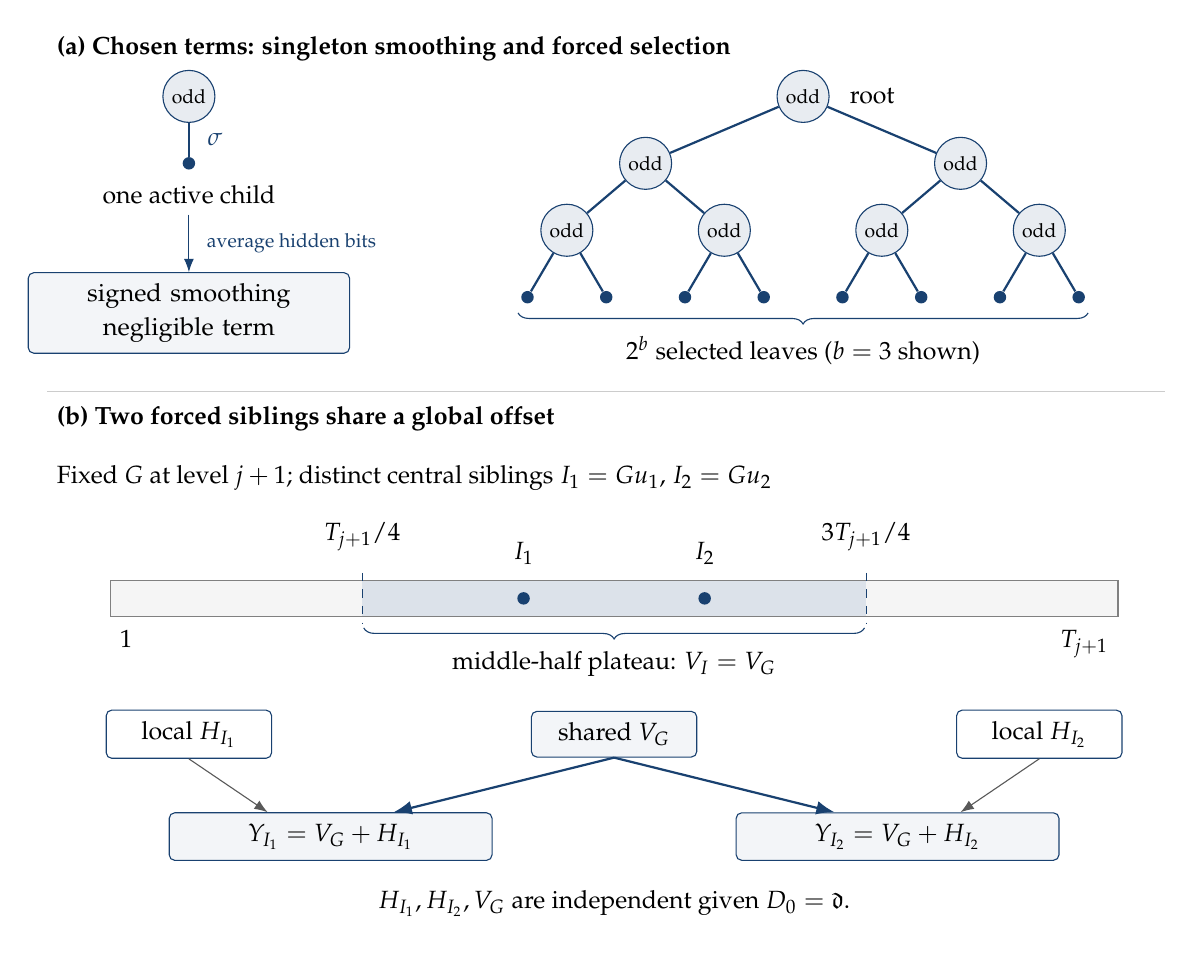
\begin{tikzpicture}[x=1cm,y=1cm,font=\small,>=Latex,
  odd/.style={circle,draw=linkblue,fill=linkblue!10,inner sep=2pt,
              minimum size=0.62cm,font=\scriptsize},
  leaf/.style={circle,fill=linkblue,inner sep=0pt,minimum size=4.5pt},
  box/.style={draw=linkblue,rounded corners=2pt,fill=linkblue!5,
              align=center,inner sep=4pt}]
  \node[anchor=west,font=\small\bfseries] at (0,0.35)
    {(a) Chosen terms: singleton smoothing and forced selection};

  \node[odd] (single-root) at (1.8,-0.25) {odd};
  \node[leaf] (single-child) at (1.8,-1.10) {};
  \draw[linkblue,thick] (single-root)--(single-child)
    node[midway,right=3pt] {$\sigma$};
  \node[align=center] at (1.8,-1.50) {one active child};
  \node[box,text width=3.8cm] (single-result) at (1.8,-3.00)
    {signed smoothing\\[1pt]
     negligible term};
  \draw[->,linkblue] (1.8,-1.75)--(single-result.north)
    node[midway,right=3pt,font=\scriptsize] {average hidden bits};

  \node[odd] (root) at (9.6,-0.25) {odd};
  \node[anchor=west] at (10.07,-0.25) {root};
  \node[odd] (a) at (7.6,-1.10) {odd};
  \node[odd] (b) at (11.6,-1.10) {odd};
  \node[odd] (aa) at (6.6,-1.95) {odd};
  \node[odd] (ab) at (8.6,-1.95) {odd};
  \node[odd] (ba) at (10.6,-1.95) {odd};
  \node[odd] (bb) at (12.6,-1.95) {odd};
  \foreach \parent/\child in {root/a,root/b,a/aa,a/ab,b/ba,b/bb}
    \draw[linkblue,thick] (\parent)--(\child);
  \foreach \parent/\xx/\yy in
    {aa/6.1/7.1,ab/8.1/9.1,ba/10.1/11.1,bb/12.1/13.1} {
    \node[leaf] (left-\parent) at (\xx,-2.80) {};
    \node[leaf] (right-\parent) at (\yy,-2.80) {};
    \draw[linkblue,thick] (\parent)--(left-\parent);
    \draw[linkblue,thick] (\parent)--(right-\parent);
  }
  \draw[decorate,decoration={brace,mirror,amplitude=4pt},linkblue]
    (5.98,-3.00)--(13.22,-3.00)
    node[midway,below=5pt,text=black] {$2^b$ selected leaves ($b=3$ shown)};

  \draw[black!20] (0,-4.00)--(14.2,-4.00);
  \node[anchor=west,font=\small\bfseries] at (0,-4.35)
    {(b) Two forced siblings share a global offset};
  \node[anchor=west] at (0,-5.10)
    {Fixed $G$ at level $j+1$; distinct central siblings $I_1=Gu_1$, $I_2=Gu_2$};
  \fill[black!4] (0.8,-6.40) rectangle (13.6,-6.85);
  \fill[linkblue!15] (4.0,-6.40) rectangle (10.4,-6.85);
  \draw[black!50] (0.8,-6.40) rectangle (13.6,-6.85);
  \draw[linkblue,dashed] (4.0,-6.30)--(4.0,-6.95);
  \draw[linkblue,dashed] (10.4,-6.30)--(10.4,-6.95);
  \node[anchor=north west] at (0.8,-6.90) {$1$};
  \node[anchor=north east] at (13.6,-6.90) {$T_{j+1}$};
  \node[anchor=south] at (4.0,-6.15) {$T_{j+1}/4$};
  \node[anchor=south] at (10.4,-6.15) {$3T_{j+1}/4$};
  \node[leaf] at (6.05,-6.625) {};
  \node[leaf] at (8.35,-6.625) {};
  \node[anchor=south] at (6.05,-6.32) {$I_1$};
  \node[anchor=south] at (8.35,-6.32) {$I_2$};
  \draw[decorate,decoration={brace,mirror,amplitude=4pt},linkblue]
    (4.02,-7.00)--(10.38,-7.00)
    node[midway,below=5pt,text=black] {middle-half plateau: $V_I=V_G$};

  \node[box,minimum width=2.1cm] (global) at (7.2,-8.35) {shared $V_G$};
  \node[box,fill=white,minimum width=2.1cm] (local1) at (1.8,-8.35)
    {local $H_{I_1}$};
  \node[box,fill=white,minimum width=2.1cm] (local2) at (12.6,-8.35)
    {local $H_{I_2}$};
  \node[box,minimum width=4.1cm] (offset1) at (3.6,-9.65)
    {$Y_{I_1}=V_G+H_{I_1}$};
  \node[box,minimum width=4.1cm] (offset2) at (10.8,-9.65)
    {$Y_{I_2}=V_G+H_{I_2}$};
  \draw[->,linkblue,thick] (global.south)--([xshift=8mm]offset1.north);
  \draw[->,linkblue,thick] (global.south)--([xshift=-8mm]offset2.north);
  \draw[->,black!65] (local1.south)--([xshift=-8mm]offset1.north);
  \draw[->,black!65] (local2.south)--([xshift=8mm]offset2.north);
  \node[align=center] at (7.2,-10.50)
    {$H_{I_1},H_{I_2},V_G$ are independent given $D_0=\mathfrak d$.};
\end{tikzpicture}
\caption{The labels ``odd'' in panel (a) describe chosen-term roles.
A singleton odd term, including at the root, is negligible after signed
smoothing.  For a remaining odd root term, selecting the first two active
children recursively forces a binary subtree with $2^b$ selected leaves
and hence $r\ge2^b$ ($b=3$ shown).  The selection is fixed by the term roles
and sibling order.  Panel (b) illustrates
\eqref{eq:prefix-offset}--\eqref{eq:global-plateau} for fixed distinct
central sibling IDs $u_1<u_2$ in one group $G$.  Conditional on the exact
typical report $D_0=\mathfrak d$, the local sums $H_{I_1},H_{I_2}$ and the
global sum $V_G$ are independent; the total offsets $Y_{I_1},Y_{I_2}$ share
$V_G$ and are estimated jointly.}
\label{fig:forced-subtree-jitter}
\end{figure}

\clearpage

First sum the extra labels so that only the forced anchor expectation remains.  Fix the forced labels and all nonleaf labels.  For an assignment $\mathbf h$ of the $e$ extra leaf labels, let $a_{\mathbf h}$ be the nonnegative expectation in \eqref{eq:anchor-extra-bound}.  At fixed bits each extra leaf has at most $L$ labels satisfying its constraint, even if several constraints share bits.  Hence
\[
 \sum_{\mathbf h}a_{\mathbf h}\le L^e\E_{\mathfrak d}f,
 \qquad
 \sum_{\mathbf h}a_{\mathbf h}^2
 \le\left(\sum_{\mathbf h}a_{\mathbf h}\right)^2
 \le L^{2e}(\E_{\mathfrak d}f)^2.
\]
This avoids a free factor $T_1$ per extra leaf.  At each positive nonroot level, there are at most $e$ occupied nonforced vertices: their descendant sets are disjoint at that level, and each contains an extra leaf and no forced leaf.  Summing their child labels costs at most
$(\prod_{j=2}^bT_j)^e$.  With the forced labels fixed, $f$ does not depend on which nonforced labels were selected, because the complete tree and every group mechanism were fixed before choosing $\mathcal S$.

\subsection{The fixed-label anchor factorization}

It remains to sum $(\E_{\mathfrak d}f)^2$ over the forced labels.  Call a forced sibling pair valid when its two labels are central and their positive difference is less than $L$.  Dropping any further order restrictions involving nonforced children can only increase this nonnegative sum.  Define the outer anchor convolution
\[
 K_{\rm out}^{\mathfrak d}(z)=\E_{\mathfrak d}\chi(z-X).
\]
Its $\ell^1$ mass is $L$, and its supremum is at most $O(L\omega^{-1}J^{-1/2})$ by the hidden root count.  Including at most $2L$ choices for the close root child, its squared sum costs
\begin{equation}\label{eq:outer-anchor-cost}
 \sum_{\substack{u_1,u_2\text{ valid root}\\\text{forced labels}}}
       K_{\rm out}^{\mathfrak d}(u_1)^2
 \le \Gamma_{\rm out},\qquad
 \Gamma_{\rm out}=O(L^3\omega^{-1}J^{-1/2}).
\end{equation}

For a fixed forced labeling, let $\mathcal G_j$ be its forced level-$(j+1)$ parents.  Each $G\in\mathcal G_j$ has two forced level-$j$ children $Gu_1(G),Gu_2(G)$ with fixed distinct labels $u_1(G)<u_2(G)$ in the middle-half interval.  For any such fixed $G$ and sibling labels $u_1<u_2$, define their joint anchor kernel by
\begin{equation}\label{eq:joint-anchor}
 \mathcal H_{j,G;u_1,u_2}^{\mathfrak d}(z_1,z_2)
 =\E_{\mathfrak d}\left[
   \chi(z_1-w_j+Y_{Gu_1})\chi(z_2-w_j+Y_{Gu_2})\right].
\end{equation}
The expectation here uses that group's global bits and the two local collections under the fixed report.  The actual $G,u_1,u_2$ select those collections; only $z_1,z_2$ are variables in the norm below.  The factor can vary with all of these fixed data.

Independence of the distinct group mechanisms conditional on $D_0=\mathfrak d$ now gives, for this fixed forced labeling,
\begin{equation}\label{eq:anchor-factorization}
 \E_{\mathfrak d}f
 =K_{\rm out}^{\mathfrak d}(h_\varnothing)
   \prod_{j=1}^{b-1}\prod_{G\in\mathcal G_j}
   \mathcal H_{j,G;u_1(G),u_2(G)}^{\mathfrak d}
       (h_{Gu_1(G)},h_{Gu_2(G)}).
\end{equation}
The group sets and sibling IDs in this identity are determined by the fixed upper labels.  In particular $\mathcal G_{b-1}$ contains the root; its interior global/local mechanism is independent of the outer mechanism defining $X$.

For fixed distinct plateau siblings, \eqref{eq:global-plateau} gives
$Y_{Gu_1}=V_G+H_{Gu_1}$ and $Y_{Gu_2}=V_G+H_{Gu_2}$.  Conditional on $\mathfrak d$, the two local hidden sums are independent of each other and of the shared global hidden sum, though their visible shifts and hidden counts can differ.  We have uniformly in the fixed data
\begin{equation}\label{eq:joint-anchor-norms}
\begin{aligned}
 \|\mathcal H_{j,G;u_1,u_2}^{\mathfrak d}\|_{\ell^1(\mathbb Z^2)}&\le L^2,\\
 \|\mathcal H_{j,G;u_1,u_2}^{\mathfrak d}\|_{\ell^\infty(\mathbb Z^2)}
 &\le C_{10}L^2\omega^{-2}(T_{j+1}t_j)^{-1/2}t_j^{-1/2}.
\end{aligned}
\end{equation}
Here $C_{10}$ is absolute.  The first bound follows by summing the two indicators before averaging.  For the supremum, first fix all global bits and bound the local average at $Gu_2$ by $O(L\omega^{-1}t_j^{-1/2})$.  This bound is uniform in the global offset, so discard that factor's constraint.  Average the other factor over its local bits and the global bits.  The latter contain at least a constant times $\omega^2T_{j+1}t_j$ hidden fair trials, giving $O(L\omega^{-1}(T_{j+1}t_j)^{-1/2})$.  Multiplication proves the displayed joint bound without treating the two offsets as independent.

Multiplying the $\ell^1$ and supremum bounds controls the squared $\ell^2$ sum.  Allowing a close child for each anchor costs at most $(2L)^2$.  Thus for fixed valid $G,u_1,u_2$,
\begin{equation}\label{eq:group-anchor-cost}
\begin{aligned}
 \sum_{\substack{z_1,z'_1,z_2,z'_2\in\mathbb Z\\
                  0<z'_1-z_1<L,\ 0<z'_2-z_2<L}}
       \mathcal H_{j,G;u_1,u_2}^{\mathfrak d}(z_1,z_2)^2
 &\le\Gamma_j,\\
 \Gamma_j&=C_{11}L^6\omega^{-2}T_{j+1}^{-1/2}t_j^{-1},
\end{aligned}
\end{equation}
with an absolute $C_{11}$ large enough for every group.

We make the order of the nested sums explicit.  For two fixed valid level-$j$ siblings $Gu_1,Gu_2$, let $\mathcal R_j(G;u_1,u_2)$ be the sum of the squares of the products of all their interior $\mathcal H$ factors, including the factor of $G$, over all valid forced descendant labelings.  Set $\mathcal R_0=1$.  Splitting the descendant labels at their first two pairs gives the exact recurrence
\begin{equation}\label{eq:anchor-sum-recursion}
\begin{aligned}
 \mathcal R_j(G;u_1,u_2)
 &=\sum_{\substack{(z_1,z'_1),(z_2,z'_2)\\
                    \text{valid at level }j}}
 \mathcal H_{j,G;u_1,u_2}^{\mathfrak d}(z_1,z_2)^2
 \prod_{v=1}^2\mathcal R_{j-1}(Gu_v;z_v,z'_v)\\
 &\le \Gamma_j\left(\sup_{G',v_1,v_2\text{ valid}}\mathcal R_{j-1}(G';v_1,v_2)\right)^2.
\end{aligned}
\end{equation}
For the inequality, first use the uniform descendant bound on the valid distinct child pairs.  Only afterward enlarge the remaining close-label sums to at most $2L$ choices and apply \eqref{eq:group-anchor-cost}.  No group estimate is invoked at coincident sibling IDs.  Iterating this inequality from the leaves upward, and finally using \eqref{eq:outer-anchor-cost}, gives
\begin{equation}\label{eq:forced-anchor-sum}
 \sum_{\text{valid forced labels}}(\E_{\mathfrak d}f)^2
 \le \Gamma_{\rm out}\prod_{j=1}^{b-1}\Gamma_j^{2^{b-j-1}}.
\end{equation}
This procedure applies a uniform bound to each actual group after its upper IDs are fixed; it does not replace the varying kernels by one stationary kernel.

\subsection{The exponent gain and closure}

Combine the extra-label reduction, \eqref{eq:forced-anchor-sum}, and the squared moment factor $(C_1r_i)^{2r}N^{-a_0dr}$.  The fixed shape and expansion counts, the powers of $L$ and $\omega^{-1}$, and the positive factor $(C_1r_i)^{2r}$ contribute $N^{o(\epsilon)}$ by Lemma~\ref{lem:scale-margins} and \eqref{eq:block-losses}.  The squared degree contribution of a branching term is therefore at most
\[
 N^{o(\epsilon)}J^{-1/2}
 \prod_{j=1}^{b-1}\bigl[T_{j+1}^{-1/2}t_j^{-1}\bigr]^{2^{b-j-1}}
 N^{-2^ba_0d}N^{-\lambda_de}.
\]
The last factor pays for every extra leaf and is at most one by \eqref{eq:score-gap}.  Using the lower bounds for $J,t_j$, the decay exponent of the remaining factors is at least
\begin{align*}
 &\epsilon/2+\sum_{j=1}^{b-1}2^{b-j-1}(\kappa_{j+1}/2+\epsilon)
       +2^ba_0d-o(\epsilon)\\
 &\qquad\ge d+(b-1)/4
       -\bigl[(2^b-1)d+3b\,2^{b-1}\bigr]\epsilon-o(\epsilon)
       >d'+.03.
\end{align*}
For this calculation, \eqref{eq:local-exponents} gives
$\kappa_{j+1}=2^{j-b}-(6\cdot2^j-2-2^{j-b})\epsilon$.  Its leading contribution at depth $j$ is
$2^{b-j-1}2^{j-b}/2=1/4$, which is the gain from the shared location of each forced sibling group.  The bound $d\le2.20+(B/4)D$ and the chosen $\epsilon$ absorb the displayed corrections and leave the strict margin over $d'=d+(b-1)/4-.05$.

For each $r<r_*$, combine the fixed-shape estimates by Cauchy--Schwarz in \eqref{eq:degree-reduction}.  The noncentral and singleton terms are at most $N^{-d'-1}$ in squared norm, and the branching terms have the margin just proved.  Summing the finitely many degree norms and the tail in \eqref{eq:tree_high} yields
\[
 \|G_+-G_-\|_{r_i}^2\le N^{-d'-.01},
\]
which proves Lemma~\ref{lem:tree-score}.

Apply Lemma~\ref{lem:clipping} to the preliminary laws $\widetilde\mu_i,\widetilde\nu_i$, their common report $D_0$, and the conditional densities \eqref{eq:conditional-densities}.  The typical report has probability $1-o(\Delta)$, \eqref{eq:tree_high} supplies $\rho=g_B$, and Lemma~\ref{lem:tree-score} supplies the density difference.  Conditioning on the common event consisting of typical metadata and $G_+\ge1/2$ gives laws $\mu_i,\nu_i$ with the required domination and score.  Each preliminary law changes by $o(\Delta)$.  The hidden-bit law was used only before this conditioning.

Together with \eqref{eq:projection_tree}, the new conditioning and failed-layout loss is at most $\Delta$ for all large instances.  The inherited loss is at most $(\prod_jT_j)E_{i-1}\le(\prod_jP_j)E_{i-1}=(\ell_i/\ell)E_{i-1}$.  Thus one may take
\[
 E_i\le\Delta+(\ell_i/\ell)E_{i-1},\qquad
 \frac{E_i}{\ell_i}\le\frac{\Delta}{\ell_i}
       +\frac{E_{i-1}}{\ell_{i-1}}\le(i+1)\Delta.
\]
The length and overlap conditions were proved in Section~\ref{sec:block}, so this completes Proposition~\ref{prop:block}.  Starting from Proposition~\ref{prop:initial} and iterating the block proves Proposition~\ref{prop:construction}.

\section{Genuine traces, exact lengths, and testing}\label{sec:transfer}

Proposition~\ref{prop:construction} now supplies the final pair and its auxiliary laws.  We first retain a one-trace bound before using product observations.  This proves the minimum-total-variation theorem independently of the sample-complexity deduction.

\begin{lemma}[Restoration and padding]\label{lem:restoration}
For the parameters in Section~\ref{sec:scales}, there are distinct words $x,y\in\{0,1\}^n$ such that, for every positive integer $m$,
\begin{equation}\label{eq:restored-product}
 \TV\bigl(\Dcal_q(x)^{\otimes m},\Dcal_q(y)^{\otimes m}\bigr)
 \le \sqrt{m n^{-d_D}}+2mn(D+1)\Delta.
\end{equation}
In particular,
\begin{equation}\label{eq:restored-single}
 \TV\bigl(\Dcal_q(x),\Dcal_q(y)\bigr)
 \le n^{-d_D/2}+2n(D+1)\Delta.
\end{equation}
\end{lemma}

\begin{proof}
Append the same arbitrary binary tail to $x_D,y_D$ to reach length $n$.  They remain distinct.  Applying the final common oracle kernel, then generating an independent trace of the known tail and concatenating it, approximates each padded $\delta$-trace law within $E_D\le n(D+1)\Delta$ in total variation.  Common padding by this kernel is the elementary monotonicity principle also used by \citet[proof of Lemma 10]{MPV2014}.

The final moment estimate, monotonicity of norms on a probability space, and $r_D\ge2$ give
\[
 H^2(\mu_D,\nu_D)
 \le\|d\nu_D/d\mu_D-1\|_{L^2(\mu_D)}^2
 \le n^{-d_D}.
\]
Tensorization and $\TV\le H$ bound the oracle product distance by $\sqrt{m n^{-d_D}}$.  Replacing each of the $m$ projected factors by its genuine law costs at most $mE_D$ for each hypothesis, by tensor telescoping.  This proves \eqref{eq:restored-product} for $\delta$.  Applying the additional deletion kernel independently to each sample proves the same bound for the requested $q$.  Taking $m=1$ gives \eqref{eq:restored-single}.
\end{proof}

\begin{proof}[Proof of Theorem~\ref{thm:tv}]
Fix any $q\in(0,1)$.  Choose $B=2$, $\zeta=1/2$, and auxiliary coefficients $c=1/(80\log2)<c_+=1/(40\log2)$ once, independently of $A$.  The setup inequality holds because its left side is $1/(20\log2)$.  The construction remains valid with these fixed parameters; its proof requires only their positivity and the stated eventual inequalities.  In this case $\delta>0$ is fixed, $D\to\infty$, and $d_D=2.20+0.20D\to\infty$.  For every fixed $A>0$, multiplying \eqref{eq:restored-single} by $n^A$ gives
\[
 n^{A-d_D/2}+2(D+1)n^{A+1-100(d_D+B+1)}\longrightarrow0.
\]
The construction is available for every sufficiently large integer $n$, not only a subsequence; its pair has length at most $n$ and common padding reaches $n$ exactly.  This proves \eqref{eq:min-tv}.  The sample-complexity conclusion follows from Theorem~\ref{thm:main}, whose proof below does not use Theorem~\ref{thm:tv}.  Indeed, $c\log(q^3\log n)\to\infty$ for any fixed admissible $c>0$.
\end{proof}

\subsection{Two-point testing with a strict exponent margin}

For two equally likely hypotheses with observation laws $P,Q$, every randomized decision rule has average success at most $(1+\TV(P,Q))/2$.  If $\varphi$ is the conditional probability of choosing the first hypothesis, its average success is
\[
 \frac12\bigl(1+\E_P\varphi-\E_Q\varphi\bigr)
 \le\frac12(1+\TV(P,Q)),\qquad 0\le\varphi\le1.
\]
This is the standard two-point comparison; trace-reconstruction versions appear in \citet[Appendix A.2]{HoldenLyons2020}.

Fix $0<c<c_+<1/(4\log2)$ and choose $B,\zeta$ so that
\[
 \alpha:=\frac{(1-\zeta)((B-1)/4-.05)}{B\log2}>c_+.
\]
The $j_0$ preliminary blocks have fixed number depending only on $B$, and therefore
\begin{equation}\label{eq:final-exponent}
 d_D=\alpha\log H_{\rm del}+O_B(1).
\end{equation}
For an absolute constant $a>0$ sufficiently small, \eqref{eq:restored-product} with $m\le a n^{d_D}$ is strictly less than $1/3$ eventually: its first term is at most $\sqrt a$, and its second is at most
\[
 2a(D+1)n^{d_D+1-100(d_D+B+1)}=o(1).
\]
Thus the maximal average success for the pair is at most $2/3$ (in fact strictly less for all sufficiently large instances).  Recall from the channel reduction in Section~\ref{sec:introduction} that $\log H_{\rm del}=\log(q^3\log n)+O(1)$ uniformly in $q$.  The strict inequality $\alpha>c_+$ and \eqref{eq:final-exponent} therefore imply
\begin{equation}\label{eq:intermediate-threshold}
 a n^{d_D}\ge n^{c_+\log(q^3\log n)}
\end{equation}
eventually.  Exact worst-case reconstruction with success $2/3$ would distinguish this pair with that success, so this proves the usual $2/3$ lower bound, with the additional margin needed next.

\subsection{Every fixed positive reconstruction success probability}

\begin{proof}[Proof of Theorem~\ref{thm:main}]
Fix $s\in(0,1]$ and $c$ as in the theorem, and retain $c_+>c$ above.  Choose a fixed positive integer $g$ such that $(2/3)^g<s$.  Put $N=\lfloor n/g\rfloor$ and construct the hard pair at length $N$ using the same requested deletion rate $q$ as the original instance.  Its working rate is still $\delta=\min(q,1/2)$.  Since
\[
 q^3\log N\sim q^3\log n\to\infty,
 \qquad \log N=\log n+O_g(1),
\]
the preceding construction and testing bounds apply to each gadget.

The exponent margin is preserved after dividing the length by $g$.  More explicitly,
\[
 \frac{(\log N)\log(q^3\log N)}
      {(\log n)\log(q^3\log n)}\longrightarrow1,
\]
so $c_+>c$ gives
\begin{equation}\label{eq:gadget-margin}
 N^{c_+\log(q^3\log N)}
 \ge n^{c\log(q^3\log n)}
\end{equation}
eventually.  This is why the strict intermediate exponent was chosen before fixing the number of gadgets.

Take $g$ independent fair choices between the two length-$N$ words, concatenate the chosen words, and append a common known tail of length $n-gN$.  This gives $2^g$ distinct length-$n$ hypotheses.  Give the estimator the stronger observation in which every trace is separated at the gadget boundaries, together with an independent trace of the tail.  Concatenation simulates the usual observation exactly.

The amplification of reconstruction difficulty using independent hard blocks also appears in \citet[Section 3.3]{MPV2014} and \citet[Section 4]{HoldenLyons2020}.  For the fixed product prior above, the following posterior calculation justifies the multiplication of optimal success probabilities.

Under the product prior, the separated data from different gadgets are independent.  Their posterior distributions factor as well: for a hypothesis vector $\theta=(\theta_1,\ldots,\theta_g)$ and separated data $z=(z_1,\ldots,z_g)$,
\[
 \Prob(\theta\mid z)=\prod_{j=1}^g\Prob(\theta_j\mid z_j).
\]
Hence the largest conditional probability of a correct joint guess is the product of the largest single-gadget posterior probabilities.  Averaging, independence of the $z_j$ shows that the optimal joint success is the product of the optimal single-gadget average successes.  The tail has the same law under every hypothesis and changes none of these posteriors.

For any positive integer sample budget $m\le n^{c\log(q^3\log n)}$, Equations~\eqref{eq:intermediate-threshold} and~\eqref{eq:gadget-margin} bound every single-gadget success by $2/3$.  The joint average success is therefore at most $(2/3)^g<s$.  When $m=0$, the posterior remains the uniform prior, so the optimal joint success is $2^{-g}\le(2/3)^g<s$.  A reconstruction procedure with worst-case success at least $s$ would have average success at least $s$ under this finite prior, a contradiction even in the stronger experiment.  No nonnegative integer budget at most the claimed threshold suffices, which implies \eqref{eq:main-bound}.
\end{proof}

\bibliographystyle{abbrvnat}
\begingroup
\small
\raggedright
\bibliography{references}
\endgroup
\end{document}
